%% LyX 2.2.0 created this file.  For more info, see http://www.lyx.org/.
%% Do not edit unless you really know what you are doing.
\documentclass[12pt,english]{report}
\usepackage{mathptmx,times}
\renewcommand{\familydefault}{\rmdefault}
\usepackage[T1]{fontenc}
\usepackage[latin9]{inputenc}
\usepackage[a4paper]{geometry}
\geometry{verbose,tmargin=2cm,bmargin=2cm,lmargin=2cm,rmargin=2cm,headheight=1cm,headsep=1cm,footskip=1cm}
\setcounter{secnumdepth}{3}
\setcounter{tocdepth}{3}
\setlength{\parskip}{\medskipamount}
\setlength{\parindent}{0pt}
\usepackage{babel}
\usepackage{verbatim}
\usepackage{float}
\usepackage{mathtools}
\usepackage{amsmath}
\usepackage{amssymb}
\usepackage{graphicx,epsfig}
\usepackage{setspace}
\usepackage{esint}
\usepackage[numbers]{natbib}
\PassOptionsToPackage{normalem}{ulem}
\usepackage{ulem}
\usepackage{nomencl}
\usepackage{epstopdf}
\usepackage{mathrsfs}
% the following is useful when we have the old nomencl.sty package
\providecommand{\printnomenclature}{\printglossary}
\providecommand{\makenomenclature}{\makeglossary}
\makenomenclature
\doublespacing
\usepackage[unicode=true,pdfusetitle,
 bookmarks=true,bookmarksnumbered=false,bookmarksopen=false,
 breaklinks=false,pdfborder={0 0 1},backref=false,colorlinks=false]
 {hyperref}
\usepackage{breakurl}

\makeatletter

%%%%%%%%%%%%%%%%%%%%%%%%%%%%%% LyX specific LaTeX commands.
%% Because html converters don't know tabularnewline
\providecommand{\tabularnewline}{\\}

%%%%%%%%%%%%%%%%%%%%%%%%%%%%%% User specified LaTeX commands.
\usepackage{tauthesis}
\usepackage[font={small,bf}, labelfont={small,bf}, margin=1cm]{caption}
\usepackage{titlesec}
\newcommand{\hsp}{\hspace{20pt}}
\titleformat{\chapter}[hang]{\Huge\bfseries}{\thechapter\hsp}{0pt}{\Huge\bfseries}
\usepackage{tikz}
\usepackage[europeanresistors,americaninductors]{circuitikz}
\usepackage{amsthm}
 
\Title{\textbf{Stability of Synchronous Generators}}
\Author{\textbf{\large Elad Venezian}}
\Year{May 2016}
\Supervisor{Prof. George Weiss}
\Department{School of Electrical Engineering}
\Degree{Master of Science in Electrical Engineering}


%%%%%%%%%%**********%%%%%%%%%%**********%%%%%%%%%%**********%%%%%%%%%%
\newtheorem{theorem}{Theorem}[section]

\newtheorem{corollary}[theorem]{Corollary}
\newtheorem{lemma}[theorem]{Lemma}

\newtheorem{proposition}[theorem]{Proposition}
\newtheorem{definition}[theorem]{Definition}
\newtheorem{example}[theorem]{Example}
\newtheorem{problem_statement}[theorem]{Problem Statement}
\newtheorem{remark}[theorem]{Remark}

\newcommand{\BE}{\begin{equation}}
\newcommand{\BEQ}[1]{\BE\label{#1}} % Changed by Olof
\newcommand{\EEQ}{\end{equation}}
\newcommand{\rfb}[1]{\mbox{\rm
   (\ref{#1})}\ifx\undefined\stillediting\else:\fbox{$#1$}\fi}
\newenvironment{matr}[1]{\left[ \begin{array}{#1}}{\end{array}
                         \right]}
\renewcommand{\cline}{{\mathbb C}}
\newcommand{\rline}  {{\mathbb R}}
\renewcommand{\l}    {{\lambda}}
\renewcommand{\L}    {{\Lambda}}
\renewcommand{\o}    {{\omega}}
\newcommand{\e}      {{\varepsilon}}
\newcommand{\half}   {{\frac{1}{2}}}
\newcommand{\m}      {{\hbox{\hskip 1pt}}}
\newcommand{\nm}     {{\hbox{\hskip -3pt}}}
\newcommand{\dd}     {{\rm d\hbox{\hskip 0.5pt}}}
\newcommand{\Amscr}  {{\mathcal{A}}}
\newcommand{\Bmscr}  {{\mathcal{B}}}
\newcommand{\Emscr}  {{\mathcal{E}}}
\newcommand{\Kmscr}  {{\mathcal{K}}}
\newcommand{\Mmscr}  {{\mathcal{M}}}
\newcommand{\Nmscr}  {{\mathcal{N}}}
\newcommand{\Xmscr}  {{\mathcal{X}}}
\newcommand{\FORALL} {{\hbox{$\hskip 11mm \forall \;$}}}
\newcommand{\rarrow} {{\rightarrow}}

\makeatother

\begin{document}

\coverpage

\titlepage

\prelimpages

\chapter*{Abstract}

Synchronous generators are an essential component of the
electric grid. Recently, the stability of the electric grid has become
an area of high interest and intensive research. One reason for that
is because the electric grid becomes more and more dependent on renewable
energy sources.

In the first part of this work we discuss the stability of a single generator connected
to an infinite bus, and show that certain reduced models fail to predict
the behavior of this system.

In the second part of this work, we investigate the stability of a microgrid composed of two identical
synchronous generators, inductive lines and resistive loads. We 
derive sufficient conditions for local exponential stability, with 
a region of attraction that includes any initial state such that the 
states of the generators are sufficiently close to each other. 

\tableofcontents{}

\textpages

\listoffigures

\listoftables

\printnomenclature{}

\chapter{Introduction\label{cha:introduction}}

The AC electricity grid was developed at the end of the XIXth century,
and has remained very similar until today. The grid is an enormously
complex nonlinear and randomly varying system for which rigorous
stability analysis is impossible. Many techniques and models that have
been developed to assess the stability of a power grid, using rigorous
modelling and system theory techniques mixed with practical shortcuts
and simplifying assumptions driven by experience, see for instance
\cite{Kundur}, \cite{GrSt2014}, \cite{SauerPai1998}, \cite{GOBS:03},
\cite{DoBull:12}.

In recent years, due to the increasing penetration of renewable energy
resources, which connect to the grid via power converters and produce
an intermittent power output, it is not clear whether the traditional
models and methods for controlling the power grid will succeed to
control it. Therefore, there is an increasing interest in the
fundamental mathematical models and stability analysis for the grid,
see for instance \cite{DoBull:12}, \cite{PoDoBu:13}, \cite{CaTa:14},
\cite{NaWe:14}, \cite{NaWe:15}, \cite{DePersiSchaft:16}.

An important concept that facilitate the integration of the renewable
energy resources into the electricity grid is the microgrid concept
\cite{GreenProdanovic:07,Schiffer_2016_survey}. A microgrid is a
localized group comprised of generation units, loads and energy
storage elements. It can possess a single point of connection to the
remaining electrical power system (grid connected mode) or work as an
independent isolated network (islanded mode). It behaves as a single
controllable generator or load from the viewpoint of the remaining
electrical system in grid connected mode. In islanded mode, the
frequency, voltage and power sharing are actively controlled within
the microgrid. Controlling the frequency and voltage and balance the
active/reactive load demand, is one of the main challenges of the
microgrid system \cite{Shafiee_2016,Zhong:13}.

The {\em synchronous generator} (SG) is the main power source of the
electricity grid. The mathematical model of a SG (see the earlier
references and in addition \cite{Walker:94}, \cite{Fitzgerald:03},
\cite{MaWe:15}, etc.) is complex and difficult to use as a component
when we model a large network. Stability analysis is usually done
either by simulation, or analytically on simplified models, in which
the SGs are connected in a simple network and each SG is represented
by reduced order equations, see for instance \cite{DoBull:12} and
\cite{PoDoBu:13}. The reduced model of a SG is often obtained by
treating the stator currents as fast variables, thus eliminating them
from the state variables via the singular perturbation approach (see,
for instance, \cite{Khalil}) and keeping only the rotor angle, the
rotor angular velocity and the rotor field as relevant state
variables, see for instance \cite{Kundur} and \cite{SauerPai1998}.

SGs have the important property that once they synchronize, they tend
to remain synchronized even without any control. This is important
attribute because the electricity grid must maintain nearly constant
frequency, and because the ability of a SG to transfer constant power
to the grid exists only when the phase difference between it and the
grid is constant. Therefore, it is desirable to know if for a given
grid which contains SGs and a loads, the SGs tend to synchronize (for
initial states in a reasonably large region) and if yes, if the grid
frequency and power flows remains stable. To simplify the stability
analysis, it is common to use the Park transformation of the voltages
and currents, that maps sinusoidal positive sequence signals into a
fixed point in the state space.

The most common reduced model, which is known as the classical model,
is a second order non linear model. The reference
\cite{DePersiSchaft:16} argues that this model is not realistic enough
and that a more complicated (but still reduced) model, which they call
{\em improved swing equation} (ISE), should be used. In this work we
show that even the model proposed in \cite{DePersiSchaft:16} is not
reliable for stability analysis, because it can't predict an unstable
behavior that is predicted by a more faithful model of the same
system.

In the second part of this work, we study the configuration of a two identical SGs
connected to a resistive load, as shown in Figure
\ref{fig:TICSGThreePhase}. These generators are driven by identical
prime movers, that have frequency droop control. Our main result is
that if the difference between the initial states of the SGs is
sufficiently small, then the state of the entire system converges at
an exponential rate to a unique stable equilibrium point in the state
space $\Xmscr$, a 7-dimensional manifold. In the manifold $\Xmscr$,
the angle difference $\delta$ between the generators is counted modulo 
$2\pi$. In some arguments we use $\rline^7$ as a state space, and then 
$\delta$ can take any real value.


%%%%%%%%%%**********%%%%%%%%%%**********%%%%%%%%%%**********%%%%%%%%%%
\begin{figure} [H]% Figure 1: tree phase TICSG system
\centering 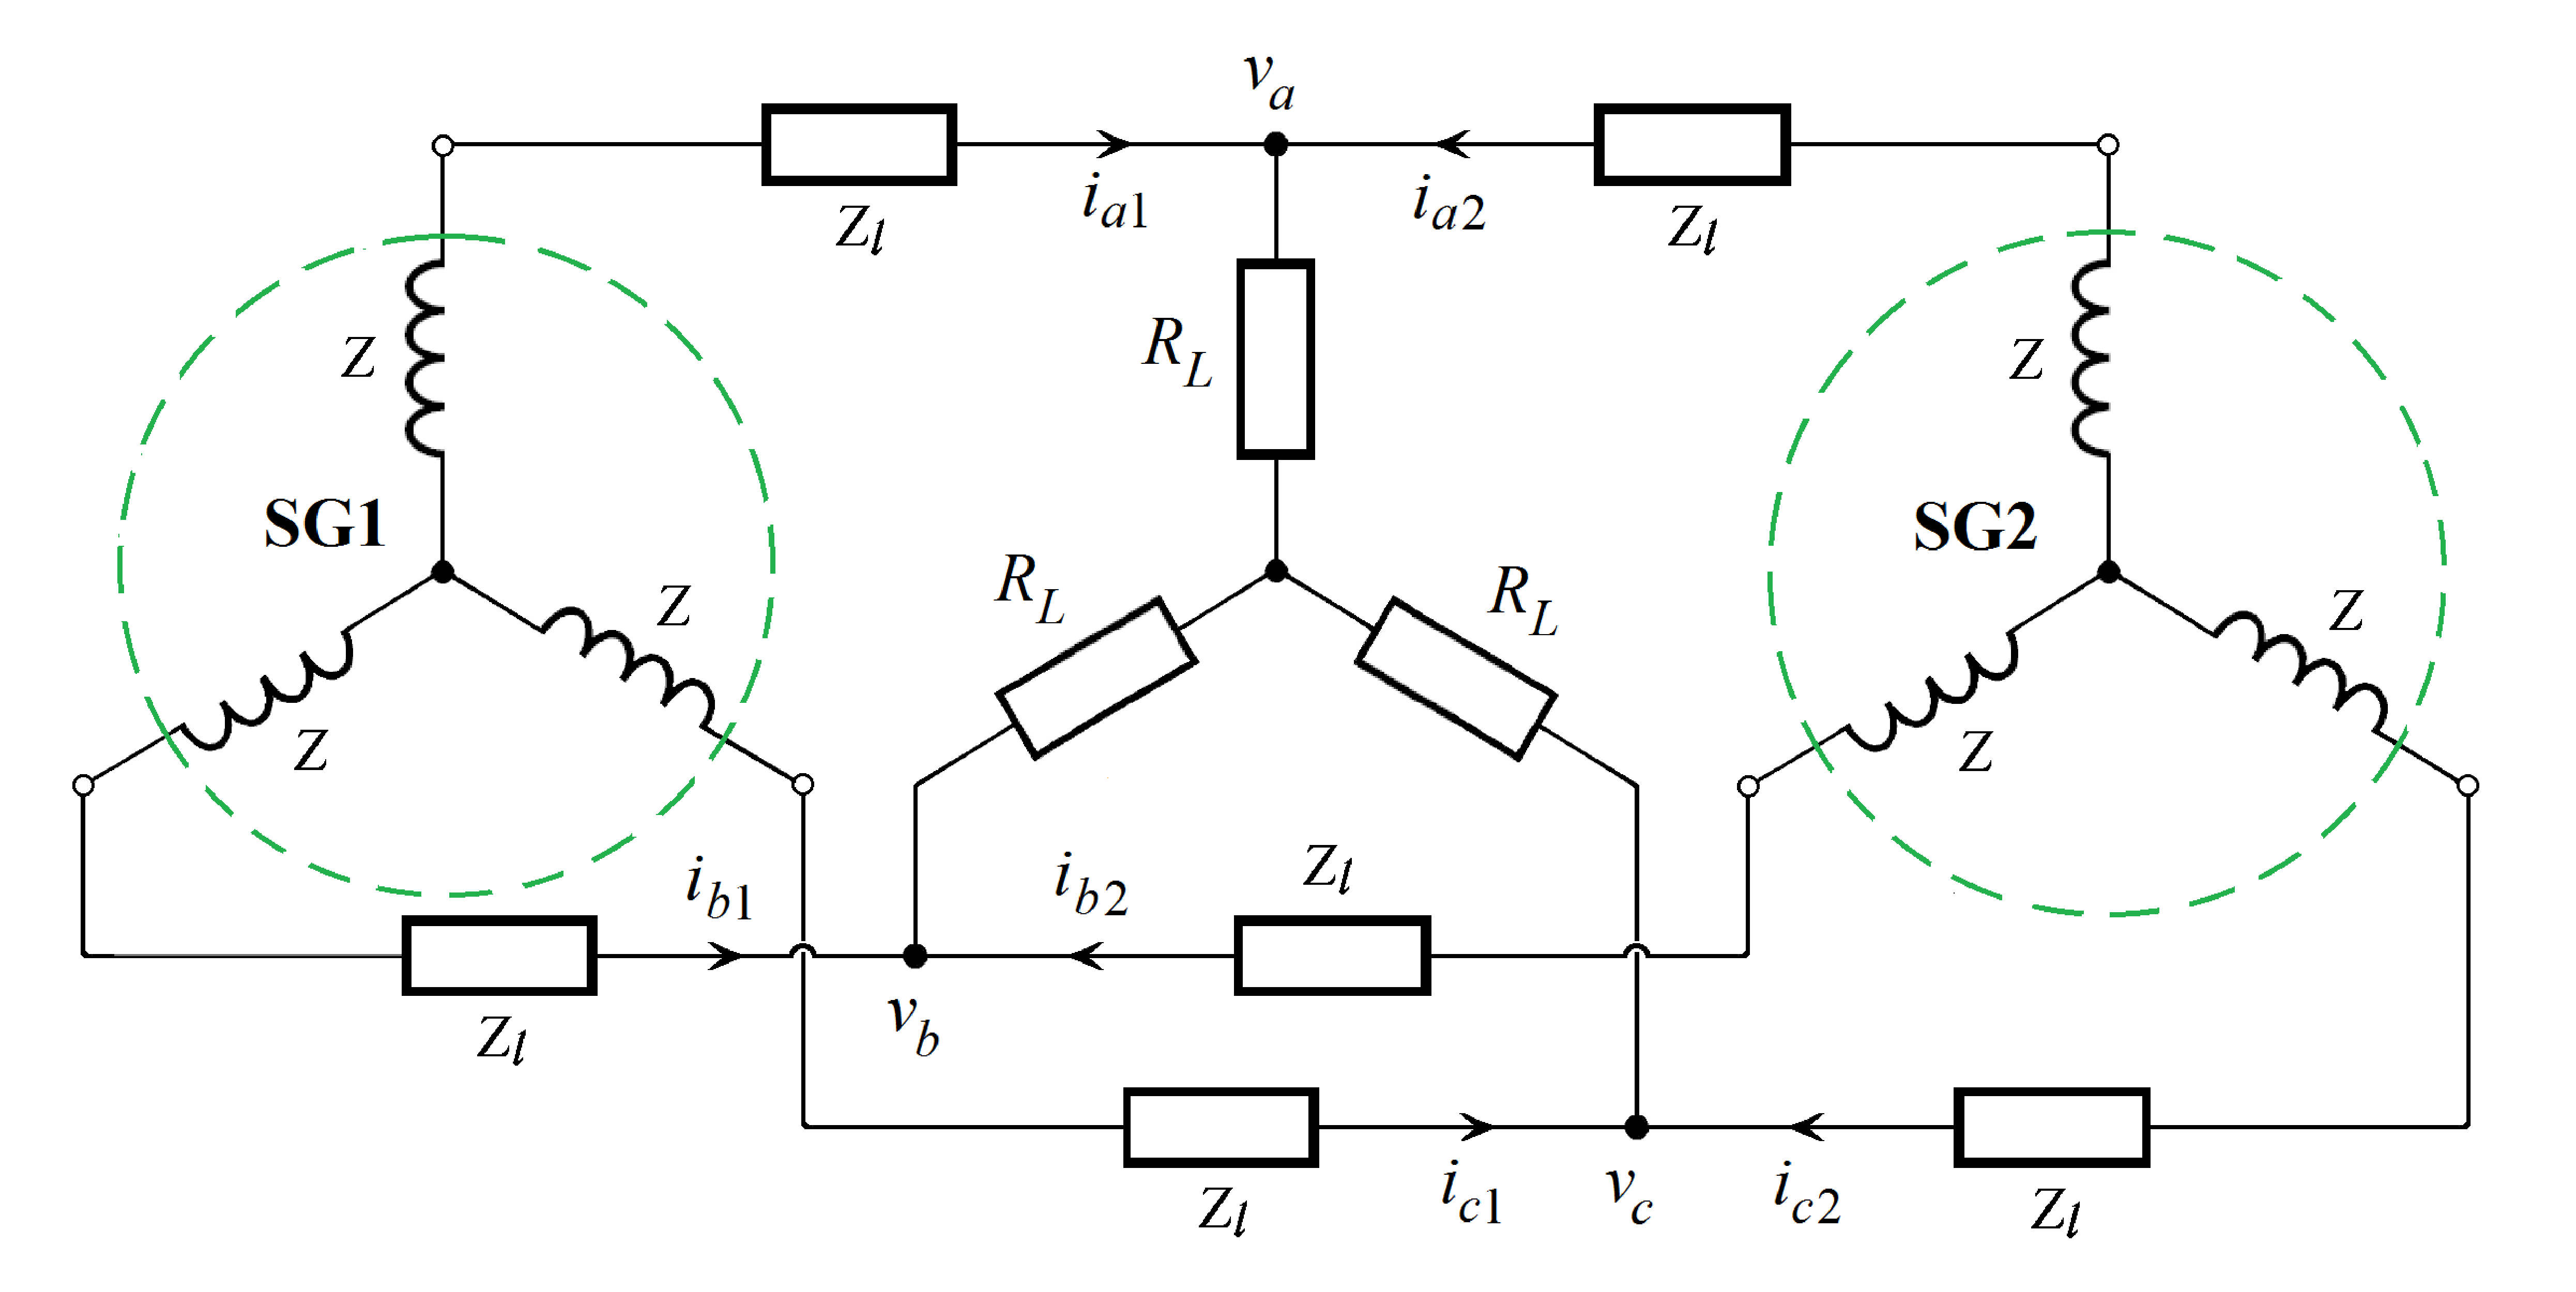
\includegraphics[width=12cm]{full_circuit_with_2_SGs}
\caption{The two identical coupled SGs (TICSG) model, showing the 
stator windings, the line impedances $Z_l$ and the load resistors 
$R_L$, but not showing the rotor windings or the prime movers.}
\label{fig:TICSGThreePhase}
\end{figure}
%%%%%%%%%%**********%%%%%%%%%%**********%%%%%%%%%%**********%%%%%%%%%%


This work has the following structure: in chapter   \ref{cha:microgrid_dynamics} third order model of a SG is presented. then, we discuss the model of a SG connected to infinite bus and having constant field current is presented. Finally, the model of {\em two identical coupled SGs} (TICSG) is described. Chapter \ref{cha:equivalence_pont}
discusses the  equilibrium point for both single SG connected to infinite bus, and the TICSG system - in particular, the existence of at last one equilibrium point
where the SGs are synchronnized (meaning that they have equal angular
velocities, angles and currents). The reduction from the model of a single SG connected to infinite bus to the second order ISE is described in \ref{cha:Model_reduction}. Simulations and local stability analysis that shows different behavior of the models are given as well. In Chapter \ref{cha:Synchronization} we analyze the stability of the TICSG system. In Section \ref{sec5} we show that 
if the SGs are synchronized, then they remain synchronized and the
system state converges to the unique equilibrium point where they are
synchronized. Section \ref{sec6} contains stability analysis for the
TICSG model. First we show that the subspace $\Emscr$ of the state
space $\rline^7$ where the generators are synchronized is locally
exponentially attractive, which means that any state trajectory that
starts sufficiently close to $\Emscr$ converges to $\Emscr$ at an
exponential rate. Then we derive results about the region of
attraction of the stable equilibrium point. We illustrate our results
by simulations in Section \ref{sec7}. In particular, we show an
example of two SGs where the region of attraction of the stable
equilibrium point contains the submanifold where the generators have
equal states (as it always does), but it does not contain all
$\Xmscr$.

\chapter{The microgrid dynamics\label{cha:microgrid_dynamics}}

In this chapter we derive the equations for system that contains  a SG. We start
with derive the equations for single SG connected to an external voltage, following the notation in \cite{ZhWe:11}, see also \cite{NaWe:15}. Later we obtain a simpler model that corresponds to constant field current. Then we derive the equations for a single SG connected to an infinite bus, following \cite{NaWe:14}, \cite{NaWe:15}. Finally, we derive the model for a microgrid comprising two identical coupled SGs (TICSG).

\section{Single generator dynamics}

The rotor of a SG is a coil on a magnetic core that spins
inside a circular cavity in the stator, having the angle $\theta$ with
respect to a reference angle, see Figure 1. We denote its self
inductance by $L_f$, its resistance by $R_f$, the voltage across its
terminals by $v_f$ and the current through it (called the field
current) by $i_f$. We assume for simplicity that $L_f$ is independent
of $\theta$ and $i_f$. The stator consists of three identical windings
that are connected in a star, with phase shifts of $120^0$ (see again
Figure 1). We consider that there is no neutral connection and no
damper windings. The stator windings can be regarded as connected
coils with self inductance $L$, mutual inductance $-M$, and resistance
$R_s$ (the parameters $L_f,R_f,L,M,R_s$ are positive). We assume no
magnetic saturation effects in the iron core and no Eddy currents. The
stator terminals are labeled with the letters $a,b,c$ and the vector
of voltages on the stator terminals is denoted by $v=\left[v_a\ v_b\
v_c\right]^\top$. We denote by $v_s$ the voltage at the unconnected 
center of the star (see Figure 1) and $v^n=[v_s\ v_s\ v_s]^\top$.
We define the vectors
$$ \widetilde{\cos}\m\theta \m=\m \left[\begin{array}{c} \cos\left(
   \theta\right)\\ \cos\left(\theta-\frac{2\pi}{3}\right)\\
   \cos\left(\theta-\frac{4\pi}{3}\right) \end{array}\right] \m,\quad
   \widetilde{\sin}\m\theta \m= \left[\begin{array}{c} \sin\left(
   \theta\right)\\ \sin\left(\theta-\frac{2\pi}{3}\right)\\ \sin\left
   (\theta-\frac{4\pi}{3}\right) \end{array}\right] \m.$$
We denote the stator fluxes by $\Phi=\left[\Phi_a\ \Phi_b\ \Phi_c
\right]^\top$, the stator currents by $i=\left[i_a\ i_b\ i_c\right]
^\top$ and the rotor current by $i_f$. 

%%%%%%%%%%**********%%%%%%%%%%**********%%%%%%%%%%**********%%%%%%%%%%
\begin{figure} % Figure 2: single generator
\centering \includegraphics[width=14cm]{SGStructure.eps}
\caption[Structure of an idealized three-phase round rotor synchronous
generator]{Structure of an idealized three-phase round rotor
synchronous generator, modified from \cite[Figure 3.4]{GrSt2014}.}
\label{fig:structOfSG} \vspace{-3mm}
\end{figure}
%%%%%%%%%%**********%%%%%%%%%%**********%%%%%%%%%%**********%%%%%%%%%%

The mutual inductance between the rotor coil and each of the stator
coils varies with the rotor angle $\theta$ as follows:
$$ \left[\begin{array}{c} M_{a,f}\\ M_{b,f}\\ M_{c,f}\end{array}
   \right] \m=\m M_{f}\widetilde{\cos}\theta \m,$$
where $M_f>0$ is a constant. Hence, the vector of flux linkages of the
stator windings is
$$ \Phi \m=\m \left[\begin{array}{ccc} L & -M & -M\\ -M & L & -M\\
   -M & -M & L \end{array}\right]i + M_f i_f\widetilde{\cos}\theta
   \m.$$
   
The equation for the rotor flux linkage is
\begin{equation}
\Phi_f=M_{af}i_a+ M_{bf}i_b+M_{cf}i_c+L_fi_f=L_fi_f+M_f\left<i,\widetilde{\cos}\theta\right>. \label{eq:fieldFlux} 
\end{equation}

Since there is no neutral line, $i_a+i_b+i_c=0$, so that the previous
equation can be rewritten as 
$$\Phi \m=\m L_s i + M_f i_f \widetilde{\cos}\theta \m,$$
where $L_s=L+M$. We will assume that the rotor current is constant
(or equivalently, the rotor is composed of a permanent magnet). The
stator voltages satisfy
\BEQ{eq:SGTerminalVlotage}
   v - v^n \m=\m -R_{s}i-\frac{\dd\Phi}{\dd t} \m=\m -R_{s}i-L_{s}
   \frac{\dd i}{\dd t} + e \m,
\end{equation}

where $e=\left[e_a\ e_b\ e_c \right] ^\top$  is the back electromotive force (EMF) due to the rotor movement given
by:

\begin{equation}
e=M_{f}i_{f}\dot{\theta}\widetilde{\sin}\theta-M_{f}\frac{d\Phi_{f}}{dt}i_{f}\widetilde{\cos}\theta.\label{eq:emf}
\end{equation}

The rotor voltage satisfies 
\begin{equation}
v_f=-R_fi_f-\frac{d\Phi_f}{dt}.\label{eq:fieldVoltage}
\end{equation}

For a SG with no load, the voltages at each terminal
will be sinusoidal functions. In order to represent the voltages and
currents in a more convenient way, we apply the Park transformation
with respect to the rotor angle:
$$ x_{dq0} \m=\m \left[\begin{array}{c} x_{d}\\ x_{q}\\ x_{0}
   \end{array}\right] \m=\m U(\theta) \left[\begin{array}{c} x_{a}\\
   x_b\\ x_c\end{array}\right] \m=\m U(\theta) x \m,$$
where $x$ is a vector in $abc$ coordinates, $x_{dq0}$
is the same vector in the $dq0$ coordinates, and $U(\theta)$ is the
following unitary matrix:
\BEQ{eq:ParkTransformation}
 U(\theta) \m=\m \sqrt{\frac{3}{2}}\left[\begin{array}{ccc}
   \cos(\theta) & \cos(\theta-\frac{2\pi}{3}) & \cos(\theta-
   \frac{4\pi}{3})\\ -\sin(\theta) & -\sin(\theta-\frac{2\pi}{3})
   & -\sin(\theta-\frac{4\pi}{3})\\ \sqrt{1/2} & \sqrt{1/2} & 
   \sqrt{1/2} \end{array}\right] \m.
\end{equation}

Applying the Park transformation to \rfb{eq:SGTerminalVlotage} 
leads to
\BEQ{aPark}
   U(\theta)(v-v^n)-U(\theta)e \m=\m -R_{s}U(\theta)i - L_s 
   U(\theta) \frac{\dd i}{\dd t} \m.
\end{equation}

Now we use that, denoting $i_{dq0}=U(\theta)i$,
$$ \frac{\dd i_{dq0}}{\dd\theta} \m=\m U(\theta)\frac{\dd i}
   {\dd\theta} + \frac{\dd U(\theta)}{\dd\theta}i \m=\m
   U(\theta)\frac{\dd i}{\dd\theta} + \left[\begin{array}{c}
   i_{q}\\ -i_{d}\\ 0 \end{array}\right].$$
This implies that \vspace{-2mm}
$$ \dot{i}_{dq0} \m=\m \frac{\dd i_{dq0}}{\dd\theta} \cdot \frac
   {\dd\theta}{\dd t} \m=\m U(\theta)\dot{i} + \o\left[\begin{array}
       {c} i_q\\ -i_d\\ 0 \end{array}\right] \m,$$
where \vspace{-2mm}
$$\o \m=\m \dot{\theta}.$$
We rewrite \rfb{aPark} as follows:
\BEQ{eq:idiqDynamics}
   L_s\frac{\dd}{\dd t}\nm\left[\nm\begin{array}{c} i_d\\ i_q\\ i_0
   \end{array}\nm\right] - L_s \o \left[\nm\begin{array}{c} i_q\\ -i_d
   \\ 0 \end{array}\nm\right] = -R_s\left[\begin{array}{c} i_d\\
   i_q\\ i_0 \end{array}\right] + \left[\nm \begin{array}{c} e_d-v_d
   \\ e_q-v_q\\ \tilde v\end{array}\nm\right],
\end{equation}
where $\tilde v=e_0-v_0+v^n_0$. Here we have used that (obviously)
$v^n_d=v^n_q=0$. Since there is no neutral connection, $i_0=0$, hence
$\tilde v=0$. Applying the Park transformation to \rfb{eq:emf} gives

\begin{equation}
\left[\begin{array}{c}
e_{d}\\
e_{q}
\end{array}\right]=-\sqrt{\frac{3}{2}}M_{f}\left[\begin{array}{c}
\frac{di_{f}}{dt}\\
\omega i_{f}
\end{array}\right].\label{eq:ed_eq}
\end{equation}

Substitute \eqref{eq:fieldFlux} into \eqref{eq:fieldVoltage}, and
applying Park's transformation yields:

$$
v_{f}=-R_{f}i_{f}-L_{f}\frac{di_{f}}{dt}-\sqrt{\frac{3}{2}}M_{f}\frac{di_{d}}{dt}.
$$

Using  \eqref{eq:idiqDynamics}  and  \eqref{eq:ed_eq}  for  $\frac{di_{d}}{dt}$
dynamics, and substituting it to the previous equation, gives:

$$
\left(1-\frac{3M_{f}^{2}}{2L_{f}L_{s}}\right)\frac{di_{f}}{dt}=\sqrt{\frac{3}{2}}\frac{M_{f}}{L_{f}}\left(\omega i_{q}-\frac{R_{s}}{L_{s}}i_{d}-\frac{v_{d}}{L_{s}}\right)-\frac{R_{f}}{L_{f}}i_{f}-\frac{v_{f}}{L_{f}}.
$$

Denote $\alpha=\left(1-\frac{3M_{f}^{2}}{2L_{f}L_{s}}\right)^{-1}>0$
and $m=\sqrt{\frac{3}{2}}M_{f}$, we have 

\begin{equation}
\frac{di_{f}}{dt}=\frac{\alpha m}{L_{f}}\left(\omega i_{q}-\frac{R_{s}}{L_{s}}i_{d}-\frac{v_{d}}{L_{s}}\right)-\frac{\alpha R_{f}}{L_{f}}i_{f}-\frac{\alpha v_{f}}{L_{f}}.\label{eq:if_dynamics}
\end{equation}

Calculate $i_{d}$ and $i_{q}$ from \eqref{eq:idiqDynamics} and \eqref{eq:ed_eq},
and substituting $\frac{di_{f}}{dt}$ from \eqref{eq:if_dynamics}
gives:

\begin{equation}
\frac{d}{dt}\left[\begin{array}{c}
i_{d}\\
i_{q}
\end{array}\right]=\omega\left[\begin{array}{c}
i_{q}\\
-i_{d}
\end{array}\right]-\frac{R_{s}}{L_{s}}\left[\begin{array}{c}
i_{d}\\
i_{q}
\end{array}\right]-\frac{m}{L_{s}}\left[\begin{array}{c}
\frac{\alpha m}{L_{f}}\left(\omega i_{q}-\frac{R_{s}}{L_{s}}i_{d}-\frac{v_{d}}{L_{s}}\right)-\frac{\alpha R_{f}}{L_{f}}i_{f}-\frac{\alpha v_{f}}{L_{f}}\\
\omega i_{f}
\end{array}\right]-\left[\begin{array}{c}
v_{d}\\
v_{q}
\end{array}\right].\label{eq:idiqDynamicsWithExIf}
\end{equation}

The rotational dynamics of the rotor is given by
\BEQ{eq:mechanicalPart}
   J\dot{\omega} \m=\m T_{m}-T_{e}-D_{p} \omega \m,
\end{equation}
where $J$ is the moment of inertia of the rotor, $T_m-D_p\o$ is is the
mechanical torque coming from the prime mover, $T_e$ is the
electromagnetic torque developed by the generator, and $D_p$ is a the
frequency droop coefficient employed in the prime movers connected to
the generators. If any viscous friction is present, it can be absorbed
into the term $D_p\o$. All the parameters $J,T_m,D_p$ are positive.
The feedback term $D_p\o$ is used in order to control the frequency of
the grid, see \cite{Kundur}, \cite{PoDoBu:13}, \cite{CaTa:14},
\cite{ZhWe:11}. $T_e$ can be found using energy consideration. The 
magnetic energy stored in the generator is
$$ E_{mag} \m=\m \half \left(\langle i,L_s i \rangle + L_f i_f^2
   \right) + M_f i_f \langle i,\widetilde{\cos}\theta \rangle \m.$$
The electromagnetic torque can be calculated as follows:
$$ T_e \m=\m \frac{\partial E_{mag}}{\partial\theta}|_{\Phi,\Phi_f
   \ const.} \m=\m - \frac{\partial E_{mag}}{\partial\theta}|_{i,
   i_f\ const.}$$
(see \cite{ZhWe:11}), whence
$$ T_e \m=\m M_f i_f \left\langle i,\frac{\dd\widetilde{\cos}\theta}
   {\dd\theta} \right\rangle \m=\m M_f i_f \langle i,\widetilde
   {\sin} \theta\rangle \m=\m -m i_f i_q \m.$$

Using \eqref{eq:idiqDynamicsWithExIf}, \eqref{eq:if_dynamics}, \eqref{eq:mechanicalPart}
and the last formula, we obtain

\begin{equation}
\begin{array}{ccc}
\frac{d}{dt}\left[\begin{array}{c}
L_{s}i_{d}\\
L_{s}i_{q}\\
L_{f}i_{f}\\
J\omega
\end{array}\right] & = & \left[\begin{array}{cccc}
-\alpha R_{s} & \alpha\omega L_{s} & \alpha mR_{f} & 0\\
-\omega L_{s} & -R_{s} & 0 & -mi_{f}\\
\frac{\alpha mR_{s}}{L_{s}} & -\alpha m\omega & -\alpha R_{f} & 0\\
0 & mi_{f} & 0 & -D_{p}
\end{array}\right]\left[\begin{array}{c}
i_{d}\\
i_{q}\\
i_{f}\\
\omega
\end{array}\right]\\
 & + & \left[\begin{array}{cccc}
-\alpha & 0 & \frac{\alpha m}{L_{f}} & 0\\
0 & -1 & 0 & 0\\
\frac{\alpha m}{L_{s}} & 0 & -\alpha & 0\\
0 & 0 & 0 & 1
\end{array}\right]\left[\begin{array}{c}
v_{d}\\
v_{q}\\
v_{f}\\
T_{m}
\end{array}\right]
\end{array}\label{eq:idiqDynamicsWithExIf}
\end{equation}

This fourth order nonlinear dynamical system represents the dynamics
of single SG, if we ignore the dynamics of the rotor the rotor angle $\theta$.

\section{Single generator with constant field current dynamics}\label{sec:singleSGFixIf}

At this sections, we assume that the rotor current is constant (which
means that the field dynamics is very fast, or equivalently, the rotor
is composed of a permanent magnet).

Assuming $\frac{di_{f}}{dt}=0$, and substituting it at \eqref{eq:idiqDynamicsWithExIf}
gives:

\begin{equation}
\frac{d}{dt}\left[\begin{array}{c}
i_{d}\\
i_{q}
\end{array}\right]=\omega\left[\begin{array}{c}
i_{q}\\
-i_{d}
\end{array}\right]-\frac{R_{s}}{L_{s}}\left[\begin{array}{c}
i_{d}\\
i_{q}
\end{array}\right]-\frac{m}{L_{s}}\left[\begin{array}{c}
0\\
\omega i_{f}
\end{array}\right]-\left[\begin{array}{c}
v_{d}\\
v_{q}
\end{array}\right]\label{eq:idiqDynamicsWithFixxIf}
\end{equation}

Using \eqref{eq:idiqDynamicsWithFixxIf} and \eqref{eq:mechanicalPart}
we obtain

\begin{equation}
\frac{d}{dt}\left[\begin{array}{c}
L_{s}i_{d}\\
L_{s}i_{q}\\
J\omega
\end{array}\right]=\left[\begin{array}{ccc}
-R_{s} & \omega L_{s} & 0\\
-\omega L_{s} & -R_{s} & -mi_{f}\\
0 & mi_{f} & -D_{p}
\end{array}\right]\left[\begin{array}{c}
i_{d}\\
i_{q}\\
\omega
\end{array}\right]+\left[\begin{array}{c}
-v_{d}\\
-v_{q}\\
T_{m}
\end{array}\right]\label{eq:SGDynamics}
\end{equation}

This Third order nonlinear dynamical system represents the dynamics
of single SG with constant field current, if we ignore the rotor angle $\theta$.

\section{Model of a single generator connected to an infinite bus }

In this subsection we develop a model for single SG with constant
field current and connected to an infinite bus, following
\cite{NaWe:14}, \cite{NaWe:15}. The infinite bus is modeled as a three
phase AC voltage source, i.e, the infinite bus is not affected by the
synchronous generator that is connected to it. The justification for
this model is that the influence of a single SG on a grid is very
small. In general, the line that connects the SG to the grid has its
impedance that can be modeled (in most cases) as a resistance and an
inductance in series, but these values can simply be added to the
parameters $R_s$ and $L_s$ of the SG.

The infinite bus voltage (at the SG terminals) is
\BEQ{eq:infBusVoltageABC}
   v \m=\m \left[\begin{array}{c} v_a\\ v_b\\ v_c \end{array}\right]
   \m=\m \sqrt{\frac{2}{3}} V\left[ \begin{array}{c} \cos(\theta_{g})
   \\ \cos(\theta_{g}-\frac{2\pi}{3})\\ \cos(\theta_{g}-\frac{4\pi}
   {3}) \end{array}\right] ,
\end{equation}
where $V$ is the grid line voltage magnitude, and $\theta_g$ is the
grid angle. Let us define the {\em power angle} $\delta$ which
represents the difference between the grid and the synchronous
generator angles: \vspace{-2mm}
$$ \delta \m=\m \theta-\theta_g \m.$$
After applying the Park transformation to \rfb{eq:infBusVoltageABC},
we get 
\BEQ{BusVoltage}
   \left[\nm\begin{array}{c} v_d\\ v_q\\ v_0 \end{array} \nm\right]
   = U(\theta)\sqrt{\frac{2}{3}}V\left[\begin{array}{c} \cos
   (\theta_g)\\ \cos(\theta_g-\frac{2\pi}{3})\\ \cos(\theta_g
   -\frac{4\pi}{3}) \end{array}\right] = -V\left[\nm \begin
   {array}{c} \sin\delta\\ \cos\delta\\ 0 \end{array}\nm\right].
\end{equation}

It is easy to see that the dynamics of $\delta$ is \vspace{-2mm}
$$\dot{\delta} \m=\m \o-\o_g \m,$$
where $\o_g$ is the grid frequency. Substituting \rfb{BusVoltage}
and the above equation into \rfb{eq:SGDynamics}, we obtain
\BEQ{eq:SGDynamicsInfBus}
   \frac{\dd}{\dd t} \left[\nm \begin{array}{c}
   L_s i_d\\ L_s i_q\\ J\o\\ \delta \end{array} \nm\right] = \left[
   \nm \begin{array}{cccc} -R_s & \o L_s & 0 & 0\\ -\o L_s & -R_s &
   -mi_f & 0\\ 0 & mi_f & -D_p & 0\\ 0 & 0 & 1 & 0 \end{array} \nm
   \right] \left[\nm \begin{array}{c} i_d\\ i_q\\ \o\\ \delta
   \end{array} \nm\right] + \left[\nm \begin{array}{c} V\sin\delta
   \\ V\cos\delta\\ T_m\\ -\o_g \end{array} \nm\right]
\end{equation}
We refer to this fourth order nonlinear dynamical system as the {\em 
fourth order model} (FOM).

\section{TICSG modeling}

In this section we develop the TICSG model that represent two 
identical SGs connected to a common resistive load, as shown in
Figure \ref{fig:TICSGThreePhase}, assuming constant field currents.
The model of each SG is as in Section \ref{sec:singleSGFixIf}.

We denote the SG rotor angles by $\theta_1$ and $\theta_2$ and
$\o_1=\dot\theta_1$, $\o_2=\dot\theta_2$. We assume that identical
prime movers act on the generators, producing the torques
$T_{m}-D_p\o_i$, $i\in\{1,2\}$. By symmetry, we assume that the
voltages at the (non-connected) midpoints of the generators and the
load are zero. We denoted the phase voltages on the load by
$v=\left[v_a\ v_b\ v_c \right]^\top$, the currents of the first
generator by $i_1=\left[i_{a1} \ i_{b1}\ i_{c1}\right]^\top$ and 
similarly for the currents of the second generator.
%by $i_2=\left[i_{a2}\ i_{b2}\ i_{c2}\right]^\top$.

In Figure \ref{fig:TICSGThreePhase} we have indicated by $Z$ the
equivalent impedance of each SG stator, $Z=sL_s+R_s$. The line that
connects the SG to the load has its impedance $Z_l$ that can be
modeled as a resistance and an inductance in series, but these values
can simply be added to the parameters $R_s$ and $L_s$ of the SG. After
this simplification, each phase of the circuit from Figure
\ref{fig:TICSGThreePhase} is as in Figure \ref{fig:TICSGOnePhase}.

%%%%%%%%%%**********%%%%%%%%%%**********%%%%%%%%%%**********%%%%%%%%%%
\begin{figure} % Figure 3: Tree phase TICSG system
\centering 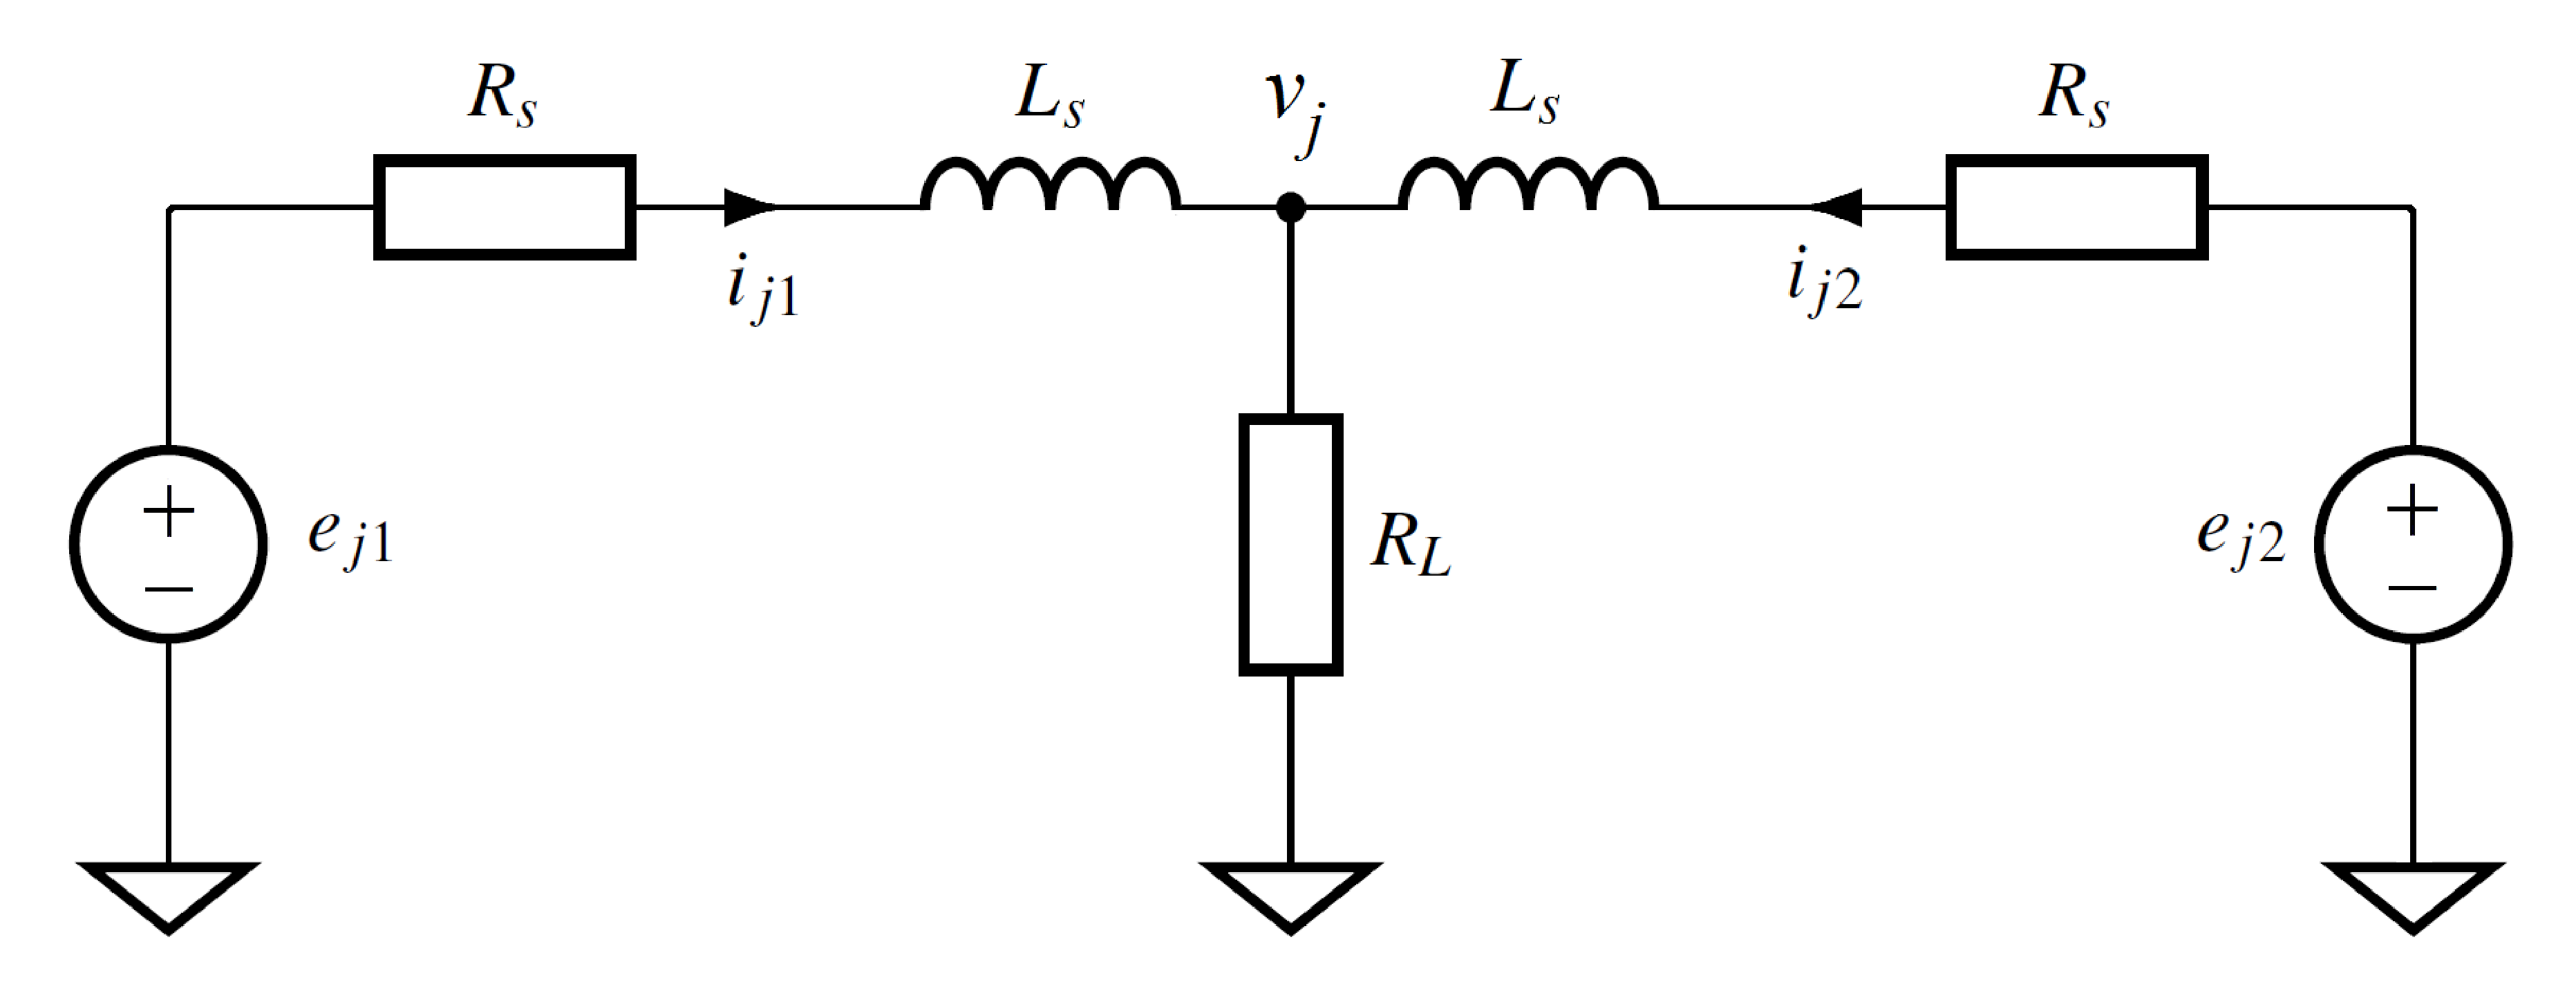
\includegraphics[width=12cm]{one_phase.eps}
\vspace{-3mm}
\caption{The TICSG model - equivalent circuit for one phase, 
$j\in\{a,b,c\}.$} \vspace{-6mm}
\label{fig:TICSGOnePhase}
\end{figure}
%%%%%%%%%%**********%%%%%%%%%%**********%%%%%%%%%%**********%%%%%%%%%%

In order to use the model \eqref{eq:SGDynamics} for each SG, we
apply the Park transformation (defined in the previous section) to the
load voltages, $\left[ v_{d1}\ v_{q1}\ v_{01}\right]^\top=U(\theta_1)
\left[v_a\ v_b\ v_c\right] ^\top$, and to the currents $\left[i_{d1}\
i_{q1}\ i_{01} \right]^\top=U(\theta_1)\left[i_{a1}\ i_{b1}\
i_{c1}\right]^\top$, and similarly for $i_2$ and $\theta_2$. From
$v=R_L(i_1+i_2)$ we get, after applying the Park transformation with
respect to $\theta_1$,
$$ \left[\begin{array}{c} v_{d1}\\ v_{q1}\\ v_{01} \end{array}
   \right] \m=\m R_L\left[\begin{array}{c} i_{d1}\\ i_{q1}\\
   i_{01} \end{array}\right] + R_L U(\theta_1)\left[\begin{array}{c}
   i_{a2}\\ i_{b2}\\ i_{c2} \end{array}\right] \m.$$
Here we express the currents of the second SG by using the inverse 
Park transformation: 
\BEQ{eq:TICSGVolAndCurr}
   \left[\begin{array}{c} v_{d1}\\ v_{q1}\\ v_{01} \end{array}\right]
   \m=\m R_{L}\left[\begin{array}{c} i_{d1}\\ i_{q1}\\ i_{01}
   \end{array}\right] + R_L U(\theta_1)U(\theta_2)^{-1}\left[
   \begin{array}{c} i_{d2}\\ i_{q2}\\ i_{02} \end{array}\right].
\end{equation}

We denote \vspace{-3mm}
$$\delta \m=\m \theta_2 - \theta_1 \m.$$

A simple computation shows that 
\BEQ{eq:ParkChangeAngle}
   U(\theta_{1})U(\theta_{2})^{-1}=\left[\begin{array}{ccc}
   \cos(\delta) & -\sin(\delta) & 0\\ \sin(\delta) & \cos(\delta) 
   & 0\\ 0 & 0 & 1 \end{array}\right].
\end{equation}

Since the SGs don't have a neutral connection, from Kirchhoff's
laws we obtain that $i_{01}=i_{02}=0$. Substituting this into
\eqref{eq:TICSGVolAndCurr} and \eqref{eq:ParkChangeAngle} shows that
$v_{01}=0$.

Substituting \eqref{eq:ParkChangeAngle} and \eqref{eq:TICSGVolAndCurr}
into \eqref{eq:SGDynamics} gives:
$$ \varLambda\dot{z}_1 \m=\m \mathcal{A}(\o_1)z_1+T_m e_3 - 
   \mathcal{B}(\delta)z_2 \m,$$
where we have denoted
 $$ z_i \m=\m \left[i_{di}\ i_{qi}\ \o_i\right]^\top,\quad 
   i\in\{1,2\},$$
$$ \varLambda \m=\m \left[\begin{array}{ccc} L_s & 0 & 0\\
   0 & L_{s} & 0\\ 0 & 0 & J \end{array}\right],$$
$$ \mathcal{A}(\o) \m=\m \left[\begin{array}{ccc}
   -R_{tot} & \o L_s & 0\\ -\o L_s & -R_{tot} & -mi_{f}\\
   0 & mi_{f} & -D_{p} \end{array}\right],$$
$$ \mathcal{B}(\delta) \m=\m \left[\begin{array}{ccc}
   R_L\cos(\delta) & -R_{L}\sin(\delta) & 0\\ R_L\sin(\delta) & 
   R_L\cos(\delta) & 0\\ 0 & 0 & 0 \end{array}\right],$$
$$e_{3}=\left[0\ 0\ 1\right]^\top, \quad R_{tot}=R_{s}+R_{L} .$$
A symmetric equation holds for the second generator:
$$ \varLambda\dot{z}_2 \m=\m \mathcal{A}(\o_{2})z_{2}+T_{m}e_{3} -
   \mathcal{B}(-\delta)z_{1} \m.$$
An additional ODE for $\delta$ is:
$$\dot{\delta} \m=\m \o_2-\o_1 \m.$$

Rewriting the entire TICSG system dynamics gives:
\begin{equation} \label{eq:TICSGDynamics}
   \frac{\dd}{\dd t}\left[\nm\nm\begin{array}{c} \varLambda z_{1}\\
   \varLambda z_{2}\\ \delta \end{array}\nm\nm\right] = \left[\nm
   \nm\begin{array}{c|c|c} \mathcal{A}(\o_1) & -\mathcal{B}(\delta)
   & 0\\ -\mathcal{B}(-\delta) & \mathcal{A}(\o_2) & 0\\ -e_{3}^T
   & e_3^T & 0 \end{array}\nm\right] \left[\nm\begin{array}{c} z_1
   \\ z_2\\ \delta \end{array}\nm\right] + T_m \left[\nm 
   \begin{array}{c} e_{3}\\ e_{3}\\ 0 \end{array} \nm\right].
\end{equation}

\begin{lemma}\label{lemma:forewordComplete}
The TICSG system is forward complete, i.e. for any initial state
$\left[ z_1^{0\top} \ z_2^{0\top} \ \delta^{0} \right]^\top \in
\mathbb{R}^7 $, the (unique) solution of the TICSG system is defined
for all $t>0$.
\end{lemma}

\begin{proof} The right hand-side of the TICSG model 
\eqref{eq:TICSGDynamics} is a locally Lipschitz function on the state
space $\rline^7$. For any initial state it follows from standard well
posedness results (see for instance \cite[Ch.~3]{Khalil}) that there
exists a unique solution $(z_1,z_2,\delta)$ for
\eqref{eq:TICSGDynamics} defined on a maximal time interval
$[0,{T_{\max}})$, with ${T_{\max}}>0$. We will show via contradiction that
${T_{\max}}=\infty$. Suppose that $T_{\max}$ is finite. For each $t\in
[0,{T_{\max}})$ define
$$ V\left(\left[\nm\begin{array}{c} z_1\\ z_2\end{array}\nm\right]
   \right) \m=\m \half \left[z_1^\top\ z_2^\top\right]\left[
   \begin{array}{cc} \varLambda & 0\\ 0 & \varLambda \end{array}
   \right]\left[ \begin{array}{c} z_1\\ z_2 \end{array}\right].$$
Then, using \eqref{eq:TICSGDynamics},
$$ \dot{V}(t) \m=\m \left[ z_1^\top\ z_2^\top\right]\left[\nm
   \begin{array}{cc} \varLambda & 0\\ 0 & \varLambda \end{array}
   \nm\right]\left[\begin{array}{c} \dot{z_1}\\ \dot{z_2}
   \end{array}\right]$$ 
$$ = \left[z_1^\top\ z_2^\top\right]\left[\nm\nm
   \begin{array}{cc} \varLambda & 0\\ 0 & \varLambda \end{array}
   \nm\nm\right] \left[\nm\nm\begin{array}{c} \varLambda^{-1}
   \left( \Amscr(\o_1)z_1-\Bmscr(\delta)z_2+T_me_3\right)
   \\ \varLambda^{-1}\left(-\mathcal{B}(-\delta)z_1+\mathcal{A}
   (\o_2)z_2+T_m e_3\right) \end{array}\nm\right].$$
Because $\mathcal{B}(-\delta) = \mathcal{B}^\top(\delta)$, we get 
$$ \begin{aligned} \dot{V}(t) =& \left(z_1^\top\mathcal{A}(\o_1)
   z_1+z_2^\top\mathcal{A}(\o_2)z_2\right) \\ &+ \left(-2z_1^\top
   \mathcal{B}(\delta)z_2 + T_mz_1^\top e_3+ T_mz_2^\top e_3\right)
   \end{aligned}$$
$$ \begin{aligned} =& \left(-R_{tot}\left(i_{d1}^2 +
   i_{q1}^2+i_{d2}^2+i_{q2}^2 \right)-D_p \left(\o_1^2+\o_2^2\right)
   \right) \\ & +2 R_L \left(-\cos(\delta)i_{d1}i_{d2}-\cos(\delta)
   i_{q1}i_{q2}-\sin(\delta)i_{q1}i_{d2}\right)\\ &+2 R_L
   \sin(\delta)i_{q2}i_{d1} + T_m(\o_1+\o_2).\end{aligned}$$
This equation can be rewritten as
$$ \dot{V}(t) \m=\m -D_p\left( \o_1^2+\o_2^2\right) + T_m(\o_1+\o_2)
   -\langle A\vec{i},\vec{i} \rangle \m,$$ 
where $\vec{i}=[i_{d1}\ i_{q1}\ i_{d2}\ i_{q2}]^\top$ and 
$$ \begin{aligned} A &=\left[\begin{array}{cc|cc} R_{tot} & 0 & R_L 
   \cos(\delta) & -R_L \sin(\delta) \\ 0 & R_{tot} & R_L R_L 
   \sin(\delta) & R_L\cos(\delta) \\ \hline R_L\cos(\delta) & R_L 
   \sin(\delta) & R_{tot} & 0 \\ -R_L \sin(\delta) & R_L\cos(\delta) 
   & 0 & R_{tot} \end{array}\right]\\ &= \left[ \begin{array}{c|c}
   A_1 & B \\ \hline B^* & A_1 \end{array} \right].\end{aligned}$$

According to the well known Schur complement condition for positive
definiteness, a symmetric matrix $X = \left[ \begin{array}{c|c} P_1 &
N \\ \hline N^* & P_2 \end{array}\right]$ is positive definite if and
only if $P_1>0$ and $\Delta=P_2-N^*P_1^{-1}N>0$. In our case clearly
$A_1>0$. Thus, in order to show that $A>0$ we only need to show that 
$A_1-B^*A_1^{-1}B>0$. By a simple computation,
$$ A_1-B^*A_1^{-1}B \m=\m \left[\begin{array}{cc}
   R_{tot}-\frac{R_L^2}{R_{tot}} & 0  \\ 
   0 & R_{tot}-\frac{R_L^2}{R_{tot}} \end{array}\right].$$
Since $R_{tot}>R_L$, we have indeed $A_1-B^*A_1^{-1}B>0$. 

From $A>0$, if either $|i_{d1}|$, $|i_{q1}|$, $|\o_1|$, $|i_{d2}|$,
$|i_{q2}|$ or $|\o_2|$ is sufficiently large, then
$\dot{V}(t)<0$. Therefore $V$ (and hence $i_{d1}$, $i_{q1}$, $\o_1$,
$i_{d2}$, $i_{q2}$ and $\o_2$ are bounded on $[0,{T_{\max}})$. Clearly
$\delta$ must also be bounded on $[0,{T_{\max}})$. Hence $(i_{d1},
i_{q1},\o_1,i_{d2},i_{q2},\o_2)$ are bounded on $[0,{T_{\max}})$, which
contradicts Theorem 3.3 (p. 94) in \cite{Khalil} (see also Corollary 
II.3 in \cite{JayWeissBS:09}). Therefore ${T_{\max}}=\infty$.
\end{proof}

%%%%%%%%%%**********%%%%%%%%%%**********%%%%%%%%%%**********%%%%%%%%%%
\chapter{The equilibrium points of the TICSG model \label{cha:equivalence_pont}}

In this chapter we study the equilibrium points of the TICSG
system \eqref{eq:TICSGDynamics}. We introduce the {\em synchronization 
subspace} of the state space $\rline^7$ by
\begin{equation} \label{eq:SyncSubspace}
   \Emscr \m=\m \left\{ \left[z_1 \ z_2 \ \delta \right]^\top\in
   \rline^7 \ |\ z_1=z_2,\ \delta = 0 \right\} \m.
\end{equation}
Clearly this is a 3-dimensional vector subspace. Similarly, we
introduce the {\em anti-synchronization space}
\begin{equation} \label{eq:AntiSyncSubspace}
   \Emscr' \m=\m \left\{ \left[z_1 \ z_2 \ \delta \right]^\top
   \ |\ z_1=z_2,\ \delta = \pi \right\} \m,
\end{equation}
which is an affine space (shifted vector subspace). Sometimes we find
it more convenient to consider the angle $\delta$ modulo $2\pi$, so
that the seventh coordinate of the state is no longer in $\rline$, but
instead in the unit circle. This new state space $\Xmscr$ is a 7
dimensional manifold, with a natural mapping from $\rline^7$ to
$\Xmscr$ (which leaves the first 6 coordinates unchanged), and the
images of $\Emscr$ and $\Emscr'$ via this mapping are 3 dimensional
submanifolds of $\Xmscr$ that we denote by $\Emscr_\Xmscr$ and
$\Emscr'_\Xmscr$, respectively. We call $\Emscr_\Xmscr$ the 
{\em symchronization manifold}.

\begin{proposition} \label{EqPointsProp1}
Any equilibrium point for the TICS system in $\Xmscr$ is either in
$\Emscr_\Xmscr$ or in $\Emscr'_\Xmscr$.
\end{proposition}

\begin{proof}
The equilibrium points are the solutions of the algebraic equation
\begin{equation} \label{eq:algebricEquation}
   \left[\nm\begin{array}{c|c|c} \Amscr(\o_1^e) & -\Bmscr(\delta^e) &
   0\\ \hline -\Bmscr(-\delta^e) & \Amscr(\o_2^e) & 0\\ \hline -e_3^T 
   & e_3^T & 0\end{array} \nm\right] \left[\nm\begin{array}{c} z_1^e
   \\ z_2^e\\ \delta^e\end{array}\nm\right] + T_m\left[\nm
   \begin{array}{c} e_{3}\\ e_{3}\\ 0 \end{array}\nm\right] = 0.
\end{equation}
It easy to see that according to the seventh line above,
\BEQ{Mitzpe_Ramon}
   \o_1^e \m=\m \o_2^e \m=\m \o^e \m.
\end{equation}
From the third and the sixth lines we have: 
$$ \left\{ \begin{array}{c} m i_f i_{q1}^e-D_p\o_1^e+T_m=0\\
   mi_f i_{q2}^e-D_p\o_2^e+T_m=0 \end{array}\right.$$
which implies
\BEQ{UNESCO}
    i_{q1}^{e} \m=\m i_{q2}^{e} \m=\m -\frac{T_m-D_p\o^e}{mi_f} 
    \m=:\m i_q^e \m.
\end{equation}
From the first, second, fourth and fifth lines:
$$ \begin{array}{c} -R_{tot}i_{d1}^e+\o^e L_s i_q^e-R_L\cos\delta^e
   i_{d2}^e+R_L\sin\delta^e i_q^e=0,\\ -\o^e L_s i_{d1}^e-R_{tot} 
   i_q^e-mi_f\o^e-R_L\sin\delta^e i_{d2}^e-R_L\cos\delta^e i_q^e=0,\\
   -R_{tot}i_{d2}^e+\o^e L_s i_q^e-R_L\cos\delta^e i_{d1}^e-R_L
   \sin\delta^e i_q^e=0,\\ -\o^e L_s i_{d2}^e-R_{tot}i_q^e-mi_f
   \o^e+R_L\sin\delta^e i_{d1}^e-R_L\cos\delta^e i_q^e=0.\end{array}$$
By denoting \vspace{-2mm}
$$ M \m=\m \left[\begin{array}{cc} -R_{tot} & -R_{L}\cos\delta^{e}\\
   -\o^e L_s & -R_L\sin\delta^e\\ -R_L\cos\delta^e & -R_{tot}\\
   R_L\sin\delta^e & -\o^e L_s \end{array}\right]$$
and 
$$ n \m=\m \left[\begin{array}{c} i_q^e\left(\o^e L_s+R_L\sin\delta^e
   \right)\\ -mi_f\o^e-i_q^e\left(R_{tot}+R_L\cos\delta^e\right)\\
   i_q^e\left(\o^e L_s-R_L\sin\delta^e\right)\\ -mi_f\o^e-i_q^e\left(
   R_{tot}+R_L\cos\delta^e\right) \end{array}\right]$$
we rewrite these lines in the following way:
\begin{equation} \label{eq:equilibrium_system}
   M\left[\begin{array}{c} i_{d1}^e\\ i_{d2}^e \end{array}\right]
   \m=\m n \m.
\end{equation}

Now, we show by contradiction that any equilibrium point must satisfy
$\sin\delta^e=0$. We use the Rouch\'e Capelli theorem: Any liner
equations system with the form $Mx=n$ has a solution if and only if
rank$\left[M|n\right]=$rank$\left[M\right]$. If we would have
$\sin\delta^e\neq 0$, then a simple calculation shows that 
rank$\left[M|n\right]=3$ must hold (see the proof at Appendix \ref{chap:AppendixProof}).

Obviously, rank$\left[M\right]\leq 2$. The Rouch\'e Capelli theorem
implies that under the previous assumption the linear equations system
\eqref{eq:equilibrium_system} does not have any solution. It proves
that if the TICSG system has an equilibrium point, it must satisfy
$\sin\delta^{e}=0$, whence $\delta^{e}=0$ or $\delta^e=\pi$
(modulo $2\pi$).

After substituting $\sin\delta^{e}=0$ and $\cos\delta^{e}=\pm 1$, the 
matrices in the equation \eqref{eq:equilibrium_system} become
$$ M = \left[\nm\nm\begin{array}{cc} -R_{tot} & \mp R_L\\ -\o^e L_s 
   & 0\\ \mp R_L & -R_{tot}\\ 0 & -\o^e L_s \end{array}\nm\nm\right],
   \ n = \left[\nm\begin{array}{c} i_q^e\o^e L_s\\ -mi_f\o^e-
   i_q^e\left(R_{tot} \pm R_L\right)\\ i_q^e\o^e L_s\\ -mi_f\o^e-
   i_q^e\left(R_{tot} \pm R_L\right) \end{array}\nm\right] \m.$$
From the first and third line above we see that $i_{d1}^e=i_{d2}^e$
must hold. Now the proposition follows from \eqref{Mitzpe_Ramon}, 
\eqref{UNESCO} and the facts that $i_{d1}^e=i_{d2}^e$ and
either $\delta^e=0$ or $\delta^e=\pi$ (modulo $2\pi$). 
\end{proof}

\begin{proposition} \label{EqPointsProp2}
The TICSG system has at least one equilibrium point on
synchronization subspace $\Emscr$ from \eqref{eq:SyncSubspace}.
\end{proposition}

\begin{proof}
We have to show that there exists $z^e=[i_d^e\ i_q^e\ \o^e]^\top\in
\rline^3$ such that the point $[{z^e}^\top\ {z^e}^\top\ 0]^\top\in
\Emscr$ is an equilibrium point of the TICSG system, i.e., it
satisfies \eqref{eq:algebricEquation}. It is easy to see that this 
happens if and only if
\begin{equation} \label{eq:equilbrium_algebric_eq}
   \left[\nm\nm\begin{array}{ccc} -R_s-2R_L & \o^e L_s & 0\\
   -\o^e L_s & -R_s-2R_L & -m i_f\\ 0 & m i_f & -D_p
   \end{array} \nm\right] \left[\nm\begin{array}{c} i_d^e\\
   i_q^e\\ \o^e \end{array} \nm\right] = \left[\nm\nm 
   \begin{array}{c} 0\\ 0\\ -T_m\end{array} \nm\nm\right]\nm\m.
\end{equation}
From \eqref{eq:equilbrium_algebric_eq} we derive a scalar equation to
determine the equilibrium velocity $\o^e$.

The first line of \eqref{eq:equilbrium_algebric_eq}
is $-\left(R_{tot}+R_L\right)i_d^e+\o^e L_{tot}i_q^e=0$, \ whence
\vspace{-1mm}
$$i_d^e \m=\m \frac{\o^e L_s}{R_{tot}+R_L} i_q^e \m.$$
Combining this with \eqref{UNESCO}, we get
\BEQ{Mosul}
   i_{d}^{e} \m=\m -\frac{\o^e L_s}{R_{tot}+R_L} \cdot \frac{T_m-D_p
   \o^e}{mi_f} \m.
\end{equation}

The second line of the matrix equation 
\eqref{eq:equilbrium_algebric_eq} is
$$ \o^{e}L_s i_d^e + \left(R_{tot} + R_L\right) i_q^e + mi_f\o^e 
   \m=\m 0 \m.$$
Substituting in this equation the expressions for $i_q^e$ 
\eqref{UNESCO} and $i_d^e$ \eqref{Mosul} yields the following cubic
equation in $\o^e$, where we denote $R_T=R_L+R_{tot}$:
$$ D_p L_s^2\o^{e3}-T_m L_s^2 \o^{e2} +\left(D_p R_T^2+m^2 i_f^2 
   R_T\right) \o^e - T_m R_T^2 \m=\m 0 \m.$$

Let us denote the polynomial of order 3 appearing above by $p$. 
Clearly \vspace{-2mm}
$$p(0) \m=\m -T_m R_T^2 \m<\m 0 \m.$$
On the other hand, we note that 
$$ p\left(\frac{T_m}{D_p}\right) \m=\m m^2 i_f^2 R_T\frac{T_m}{D_p} 
   \m>\m 0 \m.$$
Hence, $p$ has at least one zero in the interval $\left(0,
\frac{T_m}{D_p}\right)$. This shows that the TICSG system has at least
one equilibrium point located on the synchronization subspace 
\eqref{eq:SyncSubspace}.
\end{proof}

Note that $\Emscr'_\Xmscr$ may also contain equilibrium points.

\begin{remark}
If we take scalar products on both sides of 
\eqref{eq:equilbrium_algebric_eq} with $z^e$, we obtain
$$ \left(R_{tot}+R_L\right)\left((i_d^e)^2+(i_q^e)^2\right) \m=\m
   \left(T_m-D_p\o^e\right)\o^e \m.$$
This equation makes perfect physical sense. Indeed, assume that there
is no actual friction in the machine, $D_{p}$ is created by feedback,
so that $T_{m}-D_{p}\omega^{e}$ is the mechanical torque applied to
one generator, and then $\left(T_{m}-D_{p}\omega^{e}\right)\omega^{e}$
is the mechanical power entering one generator. On the other hand, it
is easy to see that $\left(R_{tot}+R_L\right)\left((i_d^e)^2+
(i_q^e)^2\right)=\left(R_s+2R_L\right)\left(i_a^2+i_b^2+i_c^2\right)$
which is exactly half of the power dissipated in all the resistors,
hence it is the electric power leaving one generator.
\end{remark}

%%%%%%%%%%**********%%%%%%%%%%**********%%%%%%%%%%**********%%%%%%%%%%
%%%%%%%%%%**********%%%%%%%%%%**********%%%%%%%%%%**********%%%%%%%%%%
\chapter{Model Reduction\label{cha:Model_reduction}}
In this chapter, we show model reduction for the FOM.
\section{The improved swing equation}

In this section, we show the relation between the ISE and the FOM. We
start with the FOM, and by a model reduction process, we get the ISE
model.  We apply ideas from singular perturbation analysis (see for
instance \cite{Khalil}). The FOM \rfb{eq:SGDynamicsInfBus} has the
following structure: \vspace{-3mm}
$$\m\ \ \Lambda \m \dot{z} \m=\m F(z) \m,$$ 
where $\Lambda$ is a diagonal $4\times 4$ matrix with positive
coefficients on the diagonal. Because the first two coefficients on
the diagonal of $\Lambda$ are equal to $L_s$, which in some sense can
be regarded as being small, we rewrite this dynamical system in the
following form:
$$ \left\{ \begin{array}{c} \dot{x} \m=\m f(x,y,\e) \m,\\
   \e\dot{y} \m=\m g(x,y,\e) \m. \end{array}\right.$$
By doing this, we have separated the state variables into a vector of 
fast variables, denoted by $y$, and another of slow variables, denoted
by $x$. Here, $\e>0$ is the small parameter.

We assuming that $\e$ is very small, meaning that for each $x$, the 
vector $y$ converges to a temporary equilibrium value (that depends on
$x$) much faster than the rate of change of $x$. In our specific case,
$\e=L_s$, $x=\left[\begin{array}{c} \o\\ \delta\end{array}\right]$ and
$y=\left[\begin{array}{c} i_d\\ i_q \end{array}\right]$. By taking the
first and second lines from \rfb{eq:SGDynamicsInfBus}, we have
$$ g(x,y,\e) \m=\m \left[\nm \begin{array}{cc} -R_s & \o L_s\\ -\o 
   L_s & -R_s \end{array}\nm\right] \left[\nm \begin{array}{c} i_d\\ 
   \i_q \end{array} \nm\right]+\left[\begin{array}{c} V\sin\delta\\ 
   V\cos\delta - mi_f\o \end{array}\right].$$
Our assumption that $\e$ is very small means that the subsystem $\e
\dot{y}=g(x,y,\e)$ is much faster than $\dot{x}=f(x,y,\e)$ and it is 
also stable, so that it will reach its temporary equilibrium almost 
instantly compared to the slow movement of $x$. The temporary 
equilibrium point $\hat{y}(x,\e)$ is the solution of $g(x,\hat y,\e)=
0$. The solution of this linear equation (in $\hat{y}$) is
$$ \hat{y} \m=\m -\left[\begin{array}{cc} -R_s & \o L_s\\
   -\o L_s & -R_s \end{array}\right]^{-1}\left[\begin{array}{cc}
   V\sin\delta\\ V\cos\delta - mi_f\o \end{array}\right]$$
$$ \m\qquad=\m \left[\begin{array}{cc} \frac{R_s V\sin\delta - L_s\o
   \left(mi_f\o - V\cos\delta\right)}{L_s^{2}\o^2+R_s^2}\\
   \frac{-R_s\left(mi_f\o - V\cos\delta\right) - L_s V\o\sin\delta}
   {L_s^2\o^2 + R_s^2} \end{array}\right] \m.$$
Assuming that $R_s$ is small so that the terms containing $R_s$ are
negligible, we obtain the following approximation of $\hat y$:
\BEQ{eq:ISEInfBusEstimatedCurrents}
   \hat{y}_{app} \m=\m \left[\begin{array}{c} \hat{i}_d\\
   \hat{i}_q \end{array}\right] \m=\m \left[\begin{array}{c}
   \frac{V\cos\delta - mi_f\o}{L_s\o}\\ -\frac{V\sin\delta}{L_s\o}
   \end{array}\right] \m.
\end{equation}

We substitute $\hat{y}_{app}$ obtained above into $\dot{x}=f(x,y,\e)$
(in place of $y$) to get the reduced model
\BEQ{eq:ISWWithConstTm}
 \left\{ \begin{array}{c} J\dot{\o}\o+D_p\o^2 \m=\m -\frac{mi_f V
   \sin\delta}{L_s}+T_m\o \m,\\ \dot{\delta} \m=\m \o-\o_g \m.
   \end{array}\right.
  \end{equation}
   
The power absorbed from the prime mover can be expressed approximately as \vspace{-2mm}
\BEQ{eq:tourqeApproximation}
P_m \m=\m (T_m-D_p \o_g)\o \m.
 \end{equation}
This crude approximation cannot be justified other than as a means to obtain the so-called improved swing equation, as we shall see below. A more precise expression of $P_m$ is 
$$P_m=(T_m-d_p\o)\o \m,$$
where $d_p>0$ is the part of $D_p$ due to the droop control of the prime mover (so that $T_m-d_p\o$ is the prime mover torque). 
 
If we express $T_m\o$ from \eqref{eq:tourqeApproximation}
and substitute into the model \eqref{eq:ISWWithConstTm}, we obtain
$$ \left\{ \begin{array}{c} J\dot{\o}\o+D_p\o(\o-\o_g) \m=\m P_m - 
   \frac{mi_f V\sin\delta}{L_s} \m,\\ \dot{\delta} \m=\m \o-\o_g \m.
   \end{array}\right.$$
This model is known as the {\em improved swing equation} (ISE), see
\cite{DePersiSchaft:16}, \cite{ZhouOhsawa2009}. Note that we did many
different approximations to derive it. The references just cited
normally assume that $P_m$ is constant, which then causes $T_m$ to be
a function of $\o$. Our perspective is to view $T_m$ as a constant
parameter.

Let us see what happens if we do not use the crude approximation
\eqref{eq:tourqeApproximation} and instead return to
\eqref{eq:ISWWithConstTm}. If we divide the first equation by $\o$ and
substitute $\dot{\o} = \ddot{\delta}$, then we obtain
\begin{equation} \label{Rishon}
   J\ddot{\delta}+D_p \dot{\delta} + \frac{mi_f V \sin \delta}{L_s 
   \left(\o_g + \dot{\delta}\right)} \m=\m T_m - D_p \o_g .
\end{equation}
This is an ugly nonlinear ODE. If $R_s=0$ then its equilibrium points
are exactly the same as for the FOM and if we approximate
$\o_g+\dot{\delta}\approx\o_g$, then we get the classical swing
equation. We think that the reduced model \eqref{Rishon} (which is
equivalent to \eqref{eq:ISWWithConstTm}) is closer to the FOM than the
ISE.

%%%%%%%%%%**********%%%%%%%%%%**********%%%%%%%%%%**********%%%%%%%%%%
\section{Simulations}

In this section we present simulations which demonstrate that the ISE
model is a good approximate model in many cases. We also show that
there are cases in which there is a significant mismatch between the
behavior suggested by the ISE model and the FOM. In each simulation
result, the behavior of $i_d$ and $i_q$ over time is described for
both the FOM and the ISE models. Note that for the ISE model, we use
\eqref{eq:ISEInfBusEstimatedCurrents} to estimate these currents. We
plot the frequency $\o$ and the power angle $\delta$ as functions of
time for these two models. In all the simulations, variables with a
hat correspond to the reduced model. All simulations assume constant
$P_m$. We redid the same simulations also under the assumption of
constant $T_m$ and the results are very similar, and not shown.

The first two simulations concern small SGs of 5KW and 1MW,
respectively, with parameters taken from \cite{Eitan}. These models
were originally meant to represent synchronverters, which are a type
of inverters, but from the point of view of the model, this does not
matter.

\subsection{5KW SG}
\vspace{-5mm}

%%%%%%%%%%**********%%%%%%%%%%**********%%%%%%%%%%**********%%%%%%%%%%
\begin{figure}[ht] 
\includegraphics[scale=0.9]{sim5KWInfBus}
\caption{Simulations for a 5KW SG connected to an infinite bus,
using both models. For $\o$ and $\delta$ the results are very 
similar.} \label{fig:InfBusOne5KWSG}
\end{figure}
%%%%%%%%%%**********%%%%%%%%%%**********%%%%%%%%%%**********%%%%%%%%%%

As shown in Figure \ref{fig:InfBusOne5KWSG}, simulations indicates
that for the 5KW SG, the behavior of the FOM and the ISE is almost the
same. Although the currents for the ISE have less ripple than for
the FOM, both models converge at the same rate with the same
oscillations to the same equilibrium point. (The parameters for this simulation can be found in the appendix,
table \ref{table:5KWSG}). 

\subsection{1MW SG}
\vspace{-4mm}
%%%%%%%%%%**********%%%%%%%%%%**********%%%%%%%%%%**********%%%%%%%%%%
\begin{figure}[ht]
\includegraphics[scale=0.9]{sim1MWInfBus}

\caption{Simulation for a 1MW SG on an infinite bus, both models}
\label{fig:InfBusOne1MWSG}
\end{figure}
%%%%%%%%%%**********%%%%%%%%%%**********%%%%%%%%%%**********%%%%%%%%%%

As shown in Figure \ref{fig:InfBusOne1MWSG}, simulations show that for
the 1MW SG, the behavior of the FOM and the ISE are still very
similar. Although the FOM currents are much more rippled than the ISE
currents, both models converge at the same rate with the same
oscillations to the same equilibrium point. (The parameters for this simulation can be found in the appendix,
table \ref{table:1MWSG}). 

\subsection{Non stable behavior of the reduced model}
\vspace{-4mm}
%%%%%%%%%%**********%%%%%%%%%%**********%%%%%%%%%%**********%%%%%%%%%%
\begin{figure}[ht]
\includegraphics[scale=0.9]{simDiffBehavior1}

\caption{A simulation example showing different behavior for the 
         FOM and the ISE reduced model for a 50 KW SG}
\label{fig:InfBusOne1DiffBehavior1}
\end{figure}
%%%%%%%%%%**********%%%%%%%%%%**********%%%%%%%%%%**********%%%%%%%%%%

As shown in Figure \ref{fig:InfBusOne1DiffBehavior1}, simulations show
that for other parameters set (The parameters for this simulation can be found in the appendix,
table \ref{table:DifferentBehaviorParamsSetSG}).  the behavior of the FOM and the ISE is significantly
different. The FOM is locally stable, since the eigenvalues of the
Jacobian around the equilibrium point are $-11.41\pm 376.9i,\ 
-508\pm 837i.$ The ISE doesn't have any equilibrium point for these
parameters. The ISE model has equilibrium points only if $ \left|
\sin\delta^e \right|= \left| \frac{P_m L_s}{mi_f V} \right| \le 1$.

%%%%%%%%%%**********%%%%%%%%%%**********%%%%%%%%%%**********%%%%%%%%%%
\subsection{An example for different regions of attraction}

\begin{figure}[ht]
\includegraphics[scale=0.9]{simDiffRegionOFAttraction}
\caption{Simulation example that shows different behavior for the 
full and the reduced models, for a 5 KW SG.}
\label{fig:InfBusOne1DiffRegionOfAttraction}
\end{figure}

As shown in Figure \ref{fig:InfBusOne1DiffRegionOfAttraction},
simulations show that for some parameters set (The parameters for this simulation can be found in the appendix,
table \ref{table:DifferentRegionOfAttraction}).  the initial condition of this simulation
is within the region of attraction of the reduced model, but outside
the region of attraction of the FOM. This causes the FOM to diverge
while the ISE converges to the equilibrium point.

%%%%%%%%%%++++++++++%%%%%%%%%%++++++++++%%%%%%%%%%++++++++++%%%%%%%%%%

\chapter{The stability of the TICSG system \label{cha:Synchronization}}

\section{The synchronized system} \label{sec5} % Section 5

If the state of the TICSG system \eqref{eq:TICSGDynamics} is in the
synchronization subspace $\Emscr$ from \eqref{eq:SyncSubspace}, it
means that the two generators are perfectly synchronized. We show that
$\Emscr$ is invariant under the flow of the system
\eqref{eq:TICSGDynamics} and the restriction of this flow to $\Emscr$
is globally asymptotically stable.

The TICSG system has the following structure: \vspace{-1mm}
$$ \tilde{\L}\m\frac{\dd}{\dd t}\left[z_1\ z_2\ \delta\right]^{\top}
   \m=\m f\left( \left[z_1\ z_2\ \delta\right]^{\top} \right) \m,$$
where $\tilde{\L}={\rm diag}\left(\L,\L,1\right)$. In order to show 
synchronization, it is convenient to introduce new 
state variables $e\in\rline^4$ and $x\in\rline^3$ by \vspace{-2mm}
$$ e \m=\m \left[ \begin{array}{c} z_2 - z_1\\ \delta \end{array} 
   \right] \m=\m \left[e_d\ e_q\ e_\o\ \delta \right]^\top$$
and \vspace{-2mm}
$$x \m=\m z_1+z_2 \m=\m \left[ x_d\ x_q\ x_\o\right]^\top .$$  

Then the TICSG model \eqref{eq:TICSGDynamics} can be rewritten as
\begin{equation} \label{eq:sync_sestem}
   \dot{e} \m=\m F(e,x) \m,\qquad \dot{x} \m=\m G(e,x) \m,
\end{equation}
for some smooth functions $F$ and $G$. From 
\eqref{eq:TICSGDynamics}, 
$$ \begin{aligned} \L(\dot{z}_2-\dot{z}_1) &=\m \Amscr(\o_2) z_2 + 
   T_m e_3-\Bmscr(-\delta)z_1\\ &\ \ -\left(\Amscr(\o_1)z_1+T_m 
   e_3-\Bmscr(\delta)z_2\right) \m.\end{aligned}$$
The detailed form of the equation $\dot e=F(e,x)$ is
$$ \begin{aligned} & \left[\begin{array}{cc} \varLambda & 0\\ 0 & 
   1 \end{array}\right] \frac{\dd}{\dd t}\left[\begin{array}{c}
   e_d\\ e_q\\ e_\o\\ \delta\end{array}\right] \m= \\ & \left[\nm
   \begin{array}{c} -R_{tot}(i_{d2}-i_{d1})+L_s(\o_2 i_{q2}-
   \o_1 i_{q1})\\ -L_s(\o_2 i_{d2}-\o_1 i_{d1})-R_{tot} (i_{q2}
   -i_{q1})-mi_f(\o_2-\o_1)\\ mi_f(i_{q2}-i_{q1})-D_p(\o_2-\o_1)
   \\ -(\o_2-\o_1) \end{array}\nm\right]\\ + & \left[\begin{array}
   {c} R_L\cos(\delta)(i_{d2}-i_{d1})-R_L\sin(\delta)(i_{q2}
   +i_{q1})\\ R_L\cos(\delta)(i_{q2}-i_{q1})+R_L\sin(\delta)(i_{d2}
   +i_{d1})\\ 0\\ 0 \end{array}\right]. \end{aligned}$$
From the trivial identity \m $(a+b)(x-y)+(a-b)(x+y)=2(ax-by)$ we
get that \vspace{-2mm}
$$ \begin{aligned} \o_2 i_{q2} -& \o_1 i_{q1} \m=\m \half\left[
   (\o_1+\o_2)(i_{q2}-i_{q1}) \right.\\ &+ \left. (\o_2-\o_1)(i_{q2}
   +i_{q1})\right] = \frac{x_\o e_q+e_\o x_q}{2} \end{aligned}$$
and the previous equation can be rewritten as \vspace{-1mm}
\BEQ{Hariri}
   \dot{e} \m=\m F(e,x) \m=\m \left[\nm\begin{array}{cc} \varLambda 
   & 0\\ 0 & 1 \end{array}\nm\right]^{-1} \left[A_e\left(e,x\right) 
   e + B_e \left(e,x\right) \right] \m,
\end{equation}
where 
$$ A_e\left(e,x\right) \m=\qquad\m$$
$$ \left[\nm\begin{array}{cccc}
   -R_{tot}+R_L\cos\delta & \frac{L_s}{2} x_{\o} & \frac{L_s}{2}
   x_q & 0\\ -\frac{L_s}{2} x_{\o} & -R_{tot} + R_L\cos\delta & 
   -\frac{L_s}{2} x_d - mi_f & 0\\ 0 & mi_f & -D_p & 0\\
   0 & 0 & 1 & 0 \end{array} \nm\right]$$ 
and
$$ B_e\left(e,x\right) \m=\m \left[\begin{array}{c} -R_L\sin(\delta)
   x_q\\ R_L\sin(\delta) x_d\\ 0\\ 0 \end{array}\right].$$
Note that the synchronization subspace $\Emscr$ from 
\eqref{eq:SyncSubspace}, in the new coordinates, becomes
$\Emscr=\left\{\left[\nm\begin{array}{c}x\\ e\end{array}\nm\right] 
\in\rline^7|\ e=0 \right\}$. We note that $F(0,x)=0$, which shows 
that $\Emscr$ is invariant.

For the $x$ dynamics we have
$$ \begin{aligned} \Lambda\dot{x} \m=\m & \Amscr(\o_1) z_1 + T_m e_3
   -\Bmscr(\delta) z_2\\ +& \Amscr(\o_2) z_2 + T_m e_3-\Bmscr
   (-\delta) z_1, \end{aligned}$$
\vspace{-2mm}
$$ \begin{aligned} &\Lambda\frac{\dd}{\dd t}\left[\begin{array}{c}
   x_{d}\\ x_{q}\\ x_{\o} \end{array}\right] = \\
   & \left[\begin{array}{c} - R_{tot}(i_{d1}+i_{d2})+L_s(\o_1 i_{q1}
   +\o_2 i_{q2})\\ -L_s(\o_1 i_{d1}+\o_2 i_{d2})-R_{tot}(i_{q1} +
   i_{q2})-m i_f(\o_1+\o_2)\\ m i_f(i_{q1}+i_{q2})-D_p(\o_1+\o_2) +
   2T_m \end{array}\right]\\ +& \left[ \begin{array}{c}
   -R_L\cos(\delta)(i_{d1}+i_{d2})-R_L\sin(\delta)(i_{q1}-i_{q2})\\
   -R_L\cos(\delta)(i_{q1}+i_{q2})+R_L\sin(\delta)(i_{d1}-i_{d2})\\
   0 \end{array}\right] \end{aligned}$$

From the trivial identity $(a+b)(x+y)+(a-b)(x-y)=2(ax+by)$ it 
follows that
$$ \begin{aligned} \o_1 i_{q1}+\o_2 i_{q2} &= \half\left[(\o_1+\o_2)
   (i_{q1}+i_{q2})+(\o_2-\o_1)(i_{q2}-i_{q1})\right]\\ & =\frac{x_o
   x_q+e_o e_q}{2} \end{aligned} $$
and similarly \vspace{-3mm}
$$ \o_1 i_{d1}+\o_2 i_{d2} \m=\m \frac{x_\o x_d+e_\o e_d}{2} \m.$$

The $x$ dynamics can be rewritten as:
$$ \dot{x}=G \left( e,x\right) \m=\m \Lambda^{-1}\left(A_x \left(e,x 
   \right) x + B_x \left( e,x\right) \right),$$
where
$$ A_x \left(e,x \right) = \left[\nm\nm\begin{array}{ccc}
   -R_{tot}-R_L\cos(\delta) & \frac{L_s}{2} x_\o & 0\\
   -\frac{L_s}{2} x_\o & -R_{tot}-R_L\cos(\delta) & -mi_f\\
   0 & mi_f & -D_p\end{array} \nm\right]$$
$$ B_x \left(e,x \right)=\left[\begin{array}{c}
   \frac{L_{s}}{2}e_{\omega}e_{q}-R_{L}\sin(\delta)e_{q}\\
   -\frac{L_{s}}{2}e_{\omega}e_{d}-R_{L}\sin(\delta)e_{d}\\
   2T_{m} \end{array}\right] \m.$$

%%%%%%%%%%**********%%%%%%%%%%**********%%%%%%%%%%**********%%%%%%%%%%
\begin{proposition} \label{megyek_Sde_Bokerbe}
The system $\dot x=G(0,x)$, with state space $\rline^3$, is 
globally exponentially stable if 
\begin{equation} \label{eq:condition_for_stable_G}
   16 R_T D_p \m>\m L_s^2 \left( \left(x_q^e\right)^2+\left( x_d^e
   \right)^2\right) \m.
\end{equation}
\end{proposition}

\medskip
\begin{proof}
We denote the state variables of this system by $x=\left[x_d\ x_q\ 
x_\o\right]^\top$. We denote $\tilde G(x)=G(0,x)$. Then
$$ \dot{x} \m=\m \tilde{G}(x) \m=\m \L^{-1} A\left( x_\o \right)x +
   \L^{-1} B \m,$$
where we denote
$$ A\left( x_\o \right) \m=\m A_x\left(0,x\right) \m=\m \left[\nm
   \begin{array}{ccc} - R_T & \frac{L_s}{2} x_\o & 0\\ -\frac{L_s}{2}
   x_\o & -R_T & -mi_f\\ 0 & mi_f & -D_p \end{array}\right]$$
and
$$ B \m=\m B_x\left(0,x \right) \m=\m \left[\begin{array}{c} 
   0\\ 0\\ 2T_m \end{array}\right].$$

Because the TICSG system has at least one equilibrium point in
$\Emscr$ (see Proposition \ref{EqPointsProp2}), using the new
coordinates there exists at least one $x^e=\left[x_d^e\ x_q^e\ 
x_\o^e\right]^\top\in\rline^3$ such that $\tilde{G}(x^e)=0$, 
in other words, 
\begin{equation} \label{eq:G_at_equilibrium}
   A(x_\o^e) x^e + B \m=\m 0 \m.
\end{equation}

In order to shift the equilibrium point into the origin, we introduce
the new coordinates
$$\hat{x} \m\coloneqq\m x-x^e \m.$$

A natural Lyapunov function candidate for this system is 
$$ V(\hat{x}) \m\coloneqq\m \half L_s\left(\hat{x}_d^2+\hat{x}_q^2
   \right)+\half J\hat{\o}^2 \m=\m \half\hat{x}^T\L\hat{x} \m.$$
It is easy to see that
$$ \half \min\left\{L_{s},J\right\}|\hat{x}|{}^{2}\leq V(\hat{x})
   \m\leq\m \frac{1}{2} \max\left\{L_{s},J\right\}|\hat{x}\m
   |^{2} \m,$$
\begin{equation} \label{eq:x_hat_dynamic}
   \dot{\hat{x}} \m=\m \dot{x} \m=\m \L^{-1} \left[ A(x_\o) x+
   B \right] \m.
\end{equation}
 
We rewrite $A(x_\o)$ as a sum of a constant symmetric matrix $R$, a
constant skew-symmetric matrix $\Delta(x_{\o}^e)$ and a 
skew-symmetric matrix $\Delta_0(\hat{x}_{\o})$:
\BEQ{EynAkev_spring}
   A(x_\o)x \m=\m \left[R+\Delta(x_\o^e)+\Delta_0(\hat{x}_\o)
   \right](\hat{x}+x^e) \m,
\end{equation}
where
$$ R \m=\m \left[\begin{array}{ccc} -R_T & 0 & 0\\
   0 & -R_T & 0\\ 0 & 0 & -D_{p}
\end{array}\right] \m,$$
$$ \Delta(\alpha) \m=\m \left[\begin{array}{ccc} 0 & \frac{L_s}{2}
   \alpha & 0\\ -\frac{L_s}{2}\alpha & 0 & -mi_f\\ 0 & mi_f & 0
   \end{array}\right] \quad (\alpha\in\rline)$$
and $\Delta_0(\alpha)$ is defined like $\Delta(\alpha)$, but with
$i_f=0$. Combining \eqref{eq:G_at_equilibrium}, 
\eqref{eq:x_hat_dynamic} and \eqref{EynAkev_spring} gives
$$ \dot{\hat{x}} \m=\m \L^{-1}\big( \left[R+\Delta(x_{\o}^e)+\Delta_0
   (\hat{x}_{\o})\right]\hat{x}+\Delta_0(\hat{x}_{\o})x^e\big)\m.$$
Using this formula, we compute the derivative of $V$ over time:
\vspace{-1mm}
$$ \dot{V}(\hat{x}) \m=\m \left\langle \frac{\partial V}{\partial
   \hat{x}},\dot{\hat{x}} \right\rangle \m=\m \left\langle \L
   \hat{x},\dot{\hat{x}} \right\rangle$$
$$ =\m \left\langle \L\hat{x},\L^{-1}\left( \left[R+\Delta(x_{\o}^e)
   +\Delta_0(\hat{x}_\o) \right]\hat{x}+\Delta_0(\hat{x}_\o)x^e
   \right) \right\rangle \m.$$
Because $\L$ is diagonal and $\Delta(\alpha),\Delta_0(\alpha)$ are
skew-symmetric, this simplifies to \vspace{-2mm}
\BEQ{Ibex}
   \dot{V}(\hat{x}) \m=\m \left\langle\hat{x},R\hat{x}+\Delta_0
   (\hat{x}_\o)x^e \right\rangle \m.
\end{equation}
It is easy to verify that
$$ \langle\hat{x},\Delta_0(\hat{x}_\o)x^e\rangle \m=\m \left[\nm 
   \begin{array}{c} \hat{x}_d\\ \hat{x}_q\\ \hat{x}_\o \end{array}\nm
   \right]^\top\left[\nm \begin{array}{ccc} 0 & \frac{L_s}{2} 
   \hat{x}_\o & 0\\ -\frac{L_s}{2}\hat{x}_\o & 0 & 0\\ 0 & 0 & 0 
   \end{array} \nm\right] \left[\nm \begin{array}{c} x_d^e\\ x_q^e\\ 
   x_\o^e \end{array} \nm\right]$$
$$ =\m \left[\nm\begin{array}{c} \hat{x}_d\\ \hat{x}_q\\ \hat{x}_\o 
   \end{array}\nm\right]^\top\left[\nm \begin{array}{ccc} 0 & 0 & 
   \frac{L_s}{4}x_q^e\\ 0 & 0 & -\frac{L_s}{4}x_d^e\\ \frac{L_s}{4}
   x_q^e & -\frac{L_s}{4}x_d^e & 0 \end{array}\nm\right] \left[\nm
   \begin{array}{c} \hat{x}_d\\ \hat{x}_q\\ \hat{x}_\o \end{array}\nm
   \right] \m=\m \hat{x}^{\top} S\hat{x} \m,$$
where $S$ is the symmetric $3\times 3$ matrix appearing above.
Combining this with \eqref{Ibex} we obtain 
$$\dot{V}(\hat{x}) \m=\m \hat{x}^{T}\left[R+S\right]\hat{x} \m,$$
where 
$$ R+S \m=\m \left[\begin{array}{ccc} -R_T & 0 & \frac{L_s}{4}
   x_q^e\\ 0 & -R_T & -\frac{L_s}{4} x_d^e\\ \frac{L_s}{4} x_q^e 
   & -\frac{L_s}{4} x_d^e & -D_p \end{array}\right].$$
Computing the eigenvalues of $R+S$ gives \m $\l_{1}=-R_T<0$,
$$ \l_{2,3} \m=\m -\frac{R_T+D_p}{2} \pm\frac{\sqrt{4\left(R_T-D_p
   \right)^2+L_s^2\left(\left(x_q^e\right)^2 + \left(x_d^e
   \right)^2\right)}}{4} \m.$$
All the eigenvalues are real. It is easy to see that the condition 
which guarantees that all the three eigenvalues are negative is
\eqref{eq:condition_for_stable_G}. When this condition holds, then
denoting $\l_{\max}=\max\left\{\l_i,\ i\in\{1,2,3\}\right\}$, we 
have $\dot{V}(\hat{x})<\l_{\max}|\hat{x}|^2$. It now follows from a
classical stability result, see for instance Theorem 4.10 (p.~154) in
\cite{Khalil}, that this system is globally exponentially stable. 
\end{proof}

Note that the last proposition implies that $x^e$ is the only 
equilibrium point of $\dot{x}=\tilde{G}(x)$, hence the TICSG system 
has exactly one equilibrium point in $\Emscr$.

%%%%%%%%%%**********%%%%%%%%%%**********%%%%%%%%%%**********%%%%%%%%%%
\section{The synchronization theorem} \label{sec6} % Section 6
 
First we prove that if the initial state of the TICSG model
\eqref{eq:TICSGDynamics} is such that $|e(0)|$ is small enough, then,
under some conditions, the two generators will synchronize, meaning
that $\lim_{t\to\infty}e(t)=0$. Then we show that the region of
attraction of the stable equilibrium in $\Emscr$ contains a
neighborhood of positive thickness of a large compact subset of 
$\Emscr$.

We recall a result from \cite{AndrieuJayawardhanaPraly,AJP_2016}. 
Consider a system of the form
\begin{equation} \label{eq:systemForm}
   \dot{e} \m=\m F\left(e,x\right),\quad \dot{x} \m=\m
   G\left(e,x\right) \m,
\end{equation}
where $e$ and $x$ are real vector valued functions of dimensions $n_e$ 
and $n_x$, respectively and $F,G\in C^2$ with $F(0,x)=0$. Let $\Kmscr$
be an invariant compact subset of $\rline^{n_e}\times\rline^{n_x}$. We
assume that the system is {\em forward complete on} $\Kmscr$, meaning
that for every $(e_0,x_0)\in\Kmscr$, the solution $e(e_0,x_0,t),\m 
x(e_0,x_0,t)$ of \eqref{eq:systemForm} exists for all $t\geq 0$. We 
denote 
$$ \Kmscr_x \m=\m \left\{x\in\rline^{n_x}\ |\ (0,x)\in\Kmscr \right\}
   \m.$$
The following properties of the system \eqref{eq:systemForm} have been
introduced in \cite{AndrieuJayawardhanaPraly} (see also 
\cite{AJP_2016}):

\subsubsection{TULES-NL (transversal uniform local exponential
stability on $\Kmscr$)} There exist positive numbers $r$, $k$ and $\l$
such that for all $(e_0,x_0)\in\Kmscr$ with $\left|e_0\right|\leq r$
and $t>0$, the solution satisfies
$$ \left|e\left(e_0,x_0,t\right)\right| \m\leq\m k\left|e_0\right| 
   e^{-\l t} \m.$$ 

\subsubsection{UES-TL (uniform exponential stability for the 
transversally linear system on $\Kmscr$)} There exist positive real 
numbers $\tilde{k}$ and $\tilde{\l}$ such that any solution $\tilde e
(e_0,x_0,t),\m\tilde x(x_0,t)$ of the transversally linear system
$$ \dot{\tilde{e}} \m=\m \frac{\partial F(e,x)}{\partial e} \left(0,
   \tilde{x}\right)\tilde e,\quad\ \dot{\tilde{x}} \m=\m \tilde{G}
   \left(\tilde{x}\right) \m=\m G\left(0,\tilde x\right)$$
satisfies, for all $e_0\in\rline^{n_e}$, $x_0\in\Kmscr_x$ and $t>0$,
$$ \left| \tilde{e}\right(\tilde{e}_0,\tilde{x}_0,t \left) \right| 
   \m\leq\m \tilde{k} e^{-\tilde\l t}\left| \tilde{e}_0\right| \m.$$ 

Notice that the solution of the transversally linear system is of the 
form \vspace{-3mm}
\BEQ{Kirkuk}
   \tilde e(\tilde e_0,\tilde x_0,t) \m=\m \Phi(\tilde x_0,t) 
   \tilde e_0 \m,
\end{equation}
where $\Phi:\rline^{n_x}\times[0,\infty)\rarrow\rline^{n_e\times 
n_e}$ is of class $C^2$.

\begin{theorem} \label{thm:TULESNL2UESTL}
Suppose that the system \eqref{eq:systemForm} satisfies the following
conditions:
\begin{enumerate}
\item \label{condition1}
There exist a positive real number $\mu$, such that: 
$$ \left|\frac{\partial F(e,x)}{\partial e}(0,x)\right| \m\leq\m \mu
   \FORALL x\in\Kmscr_x \m.$$

\item \label{ugly_integral}
There exists a matrix $Q>0$, such that the function 
$P:\Kmscr_x\to\rline^{n_e\times n_e}$ given by
\BEQ{simhat_tora}
   P\left(\tilde{x}_0\right) \m=\m \lim_{T\to\infty} \int_0^T 
   \Phi(\tilde{x}_0,s)^\top Q \m\Phi(\tilde{x}_0,s) \dd s
\end{equation}
exists, where $\Phi$ is as in \eqref{Kirkuk} 
(\cite{AndrieuJayawardhanaPraly} shows that $P$ always exists for 
UES-TL systems that satisfy condition 1).

\item \label{many_bounds}
There exist positive numbers $\eta$ and $c$ such that, for all 
$(e,x)\in\Kmscr$ with $|e|<\eta$,
$$ \left| \frac{\partial P}{\partial x}(x)\right| \m\leq\m c,
   \quad\left| \frac{\partial G}{\partial e}(e,x)\right| 
   \m\leq\m c \m,$$
$$ \quad  \left| \frac{\partial^2 F}{\partial e \partial e}(e,x)
   \right| \le c, \quad  \left| \frac{\partial^2 F}{\partial x 
   \partial e}(e,x)\right| \m\leq\m c\m.$$
\end{enumerate}

Then the UES-TL property implies the TULES-NL property for this 
system.
\end{theorem}

\medskip
This theorem follows from Propositions 2, 3 and Comment 2 in
\cite{AndrieuJayawardhanaPraly}. [check] ??? Still at the general
level of \eqref{eq:systemForm}, we have:

\begin{proposition} \label{Nahal_Zin}
Suppose that the system \eqref{eq:systemForm} is such that $\dot{
\tilde x}=\tilde{G}(\tilde{x})$ is globally exponentially stable
on $\Kmscr_x$, with the equilibrium point $x^e\in\Kmscr_x$. Moreover,
we assume that the matrix $\frac{\partial F}{\partial e}(0,x^e)$ 
is stable (Hurwitz). Then for every compact set $K_x$ contained in the
interior of $\Kmscr_x$ there exists $\e>0$ such that the set
$$ K(\e) \m=\m \left\{ (e,x)\in\rline^{n_e}\times\rline^{N_x}\ |\
   |e|\leq\e\m,\ x\in K_x \right\}$$
is contained in the region of attraction of the equilibrium point
$(0,x^e)$ of \eqref{eq:systemForm}.
\end{proposition}

\begin{proof} It is easy to see that $(0,x^e)$ is an exponentially 
stable equilibrium point for the system \eqref{eq:systemForm} (because
its linearization is Hurwitz). Let $\Nmscr$ be an open neighborhood of
$(0,x^e)$ contained in its region of attraction. For each $x_0\in K_x$
there exists $t>0$ such that $x(0,x_0,t)\in\Nmscr$. Taking preimage
through the flow, it follows that there exists an open neighborhood
$\Mmscr(x_0)$ of $(0,x_0)$ contained in the region of attraction of
$(0,x^e)$. We can find an open neighborhood $\tilde {\Mmscr}(x_0)$ of
$x_0$ and a number $\e(x_0)>0$ such that \vspace{-2mm}
$$ \m\ \{e\in\rline^{n_e}\m|\ |e|<\e(x_0)\}\times\tilde{\Mmscr}(x_0) 
   \m\subset\m \Mmscr(x_0) \m.$$
All the sets $\tilde\Mmscr(x_0)$ (for all $x_0\in K_x$) are an open 
covering of the compact set $K_x$. We extract a finite covering 
$\tilde\Mmscr(\xi_1),\ldots\ \tilde\Mmscr(\xi_n)$ of $K_x$, and we 
take
$$\e \m=\m \min\{\e(\xi_j)\ |\ j\in\{1,\ldots n\} \m,$$
then clearly the statement in the proposition holds.
\end{proof} 

Now we return to our TICSG model. We will use Theorem
\ref{thm:TULESNL2UESTL} to show that the TICSG system has the TULES-NL
property.

We start with computing $\frac{\partial F(e,x)}{\partial e}(0,
x)$. Using \eqref{Hariri} we can express $F$ as composed of two 
functions $F_\zeta$ and $F_\delta$:
$$ \begin{aligned} F \m=\m \left[\begin{array}{cc} F_\zeta \\ 
   F_\delta \end{array}\right] &= \left[\begin{array}{cc}
   \L & 0\\ 0 & 1 \end{array}\right]^{-1} \left[\begin{array}{cc}
   A_{e_z}(x,\delta) & 0\\ e_3^\top & 0 \end{array}\right] \left[
   \begin{array}{cc} e_\zeta \\ \delta \end{array}\right]\\ &+ 
   \left[\begin{array}{cc} \L & 0\\ 0 & 1 \end{array}\right]^{-1}
   B_e\left(x,\delta\right) \m,\end{aligned}$$
where $A_e(x,\delta)=\left[\nm\begin{array}{cc} A_{e_z}(x,\delta) 
& 0\\ e_3^\top & 0\end{array}\nm\right]$ and $e_\zeta=\left[e_d \ 
e_q \ e_\o \right]^\top$,
$$ \frac{\partial F(e,x)}{\partial e}(0,x) \m=\m \left[
   \begin{array}{cccc} \frac{\partial F_\zeta}{\partial e_\zeta} 
   & \frac{\partial F_\zeta}{\partial \delta} \\ \frac{\partial
   F_\delta}{\partial e_\zeta}  & \frac{\partial F_\delta}
   {\partial \delta} \end{array}\right].$$
We have 
$$ \begin{aligned} &\frac{\partial F_\zeta}{\partial e_\zeta}(0,x)
   \m=\m \L^{-1}A_{e_z}(x,0)\\ &=\L^{-1}\left[\begin{array}{ccc} 
   -R_{tot}+R_L & \frac{L_s}{2}x_{\o} & \frac{L_s}{2} x_q \\ 
   -\frac{L_s}{2}x_{\o} & -R_{tot} + R_L & -\frac{L_s}{2} x_d-mi_f
   \\ 0 & mi_f & -D_p \end{array}\right],\end{aligned}$$
$$ \begin{aligned} \frac{\partial F_\zeta}{\partial \delta} & =  
   \L^{-1} \frac{\partial F_\zeta}{\partial \delta}\left( 
   A_{e_\zeta}(x,\delta) \right)e_\zeta + \frac{\partial F_\zeta}
   {\partial \delta}\left(B_e(x,\delta)\right) \end{aligned}$$
$$ \frac{\partial F_\zeta}{\partial \delta}(0,x) \m=\m \left[
   \begin{array}{ccc} -R_L x_q\\ R_L x_d\\ 0\end{array}\right],
   \quad \frac{\partial F_\delta}{\partial e_\zeta} \m=\m 
   e_3^\top,\quad \frac{\partial F_\delta}{\partial \delta}
   \m=\m 0 \m.$$
Putting it all together,
\begin{equation} \label{eq:AOft}
   \frac{\partial F(e,x)}{\partial e}(0,x) = \left[\nm
   \begin{array}{cccc} -\frac{R_s}{L_s} & \frac{x_{\o}}{2} & 
   \frac{x_q}{2} & -\frac{R_L}{L_s} x_q\\ -\frac{x_{\o}}{2} &
   -\frac{R_s}{L_s} & -\frac{x_d}{2}-\frac{mi_f}{L_s} & 
   \frac{R_L}{L_s} x_d\\ 0 & \frac{mi_f}{J} & -\frac{D_p}{J} 
   & 0\\ 0 & 0 & 1 & 0 \end{array} \nm\right].
\end{equation}

\begin{theorem} \label{theorem:TICSGSync}
Assume that the TICSG system satisfies condition 
\eqref{eq:condition_for_stable_G}, \vspace{-3mm}
\begin{equation} \label{eq:eLinearizationLimit}
   A \m=\m \frac{\partial F}{\partial e}(0,x^e)
\end{equation}
is a stable (Hurwitz) matrix (condition
\eqref{eq:condition_for_stable_G} implies that the limit exists) and
moreover, there exist positive numbers $\eta$ and $c$ such that for
all $(e,x)\in\Kmscr$ with $|\e|<\eta$,
$$\left| \frac{\partial P}{\partial x}(x)\right| \m\leq\m c,$$
where $P$ is defined by \eqref{simhat_tora}. 

Then there exist strictly positive real numbers $r$, $k$ and $\l$ such
that for all $\left(e_0, x_0, t\right)$ where $\left|e_0\right|\leq r$
and the solution satisfies $\left| e\left( e_0,x_0,t\right)\right|\leq
k\left|e_0\right|e^{-\l t}$. Namely the manifold $\Emscr$ is
exponentially stable locally in $e$, uniformly in $x$.
\end{theorem}
 
\begin{proof}
We show that the TICSG system has the UES-TL property, and then by
applying theorem \ref{thm:TULESNL2UESTL}, we will show that it has
the TULES-NL property.

As we showed in Lemma \ref{lemma:forewordComplete}, the TICSG system
is forward complete. We need to show that the system
$$ \dot{\tilde{e}} \m=\m \frac{\partial F}{\partial e}(0,\tilde{x})
   \tilde{e}$$
is globally exponentially stable. Note that this is a linear time
varying system.

We use the following result from \cite[Theorem 4.2.7]
{SchovanecGilliam1999}:

\begin{proposition}\label{proposition:LTVStability}
Let $A$ be a stable (Hurwitz) matrix and let $\Pi$ be a
continuous square matrix-valued function on the interval
$[0,\infty)$. Suppose that
$$\intop_0^\infty \left|\Pi(t)\right| \dd t \m<\m \infty \m.$$
Then the solution of $\dot{x}(t)=[A+\Pi(t)]x(t)$ is globally exponentially
asymptotically stable.
\end{proposition}
 
Because Theorem \ref{theorem:TICSGSync} requires condition
\eqref{eq:condition_for_stable_G}, then the system $\tilde{x}=
\tilde{G}(\tilde{x})$ is exponentially stable and hence $A =
\lim_{t \to \infty}\frac{\partial F}{\partial e}(0,\tilde{x}^e)$
exists.  It imply that the matrix $\frac{\partial F}{\partial
e}(0,\tilde{x}^e)$ can be represented as $\frac{\partial F}{\partial
e}(0,\tilde{x}^e) = \left(A+P(t)\right)$ where $P(t)$ converges
exponentially to zero. The limit matrix is
$$ A \m=\m \left[\begin{array}{cccc} -\frac{R_{s}}{L_s} & 
   \frac{x^e_\o}{2} & \frac{x^e_q}{2} & -\frac{R_L}{L_s} x^e_q\\
   -\frac{x^e_\o}{2} & -\frac{R_s}{L_s} & -\frac{x^e_d}{2}-\frac
   {mi_f}{L_s} & \frac{R_L}{L_s} x^e_d\\ 0 & \frac{mi_f}{J} & 
   -\frac{D_p}{J} & 0\\ 0 & 0 & 1 & 0 \end{array}\right]$$
and this should be stable, according to condition
\eqref{eq:eLinearizationLimit}. This shows that proposition
\ref{proposition:LTVStability} holds and the system
$$ \dot{\tilde{e}}=\frac{\partial F}{\partial e}(0,\tilde{x})
   \tilde{e}$$
is globally exponentially stable. This proves that the TICSG system
is UES-TL. 

Both $F$ and $G$ are $C^\infty$. In addition, as shown at the proof of
Lemma \ref{lemma:forewordComplete}, $\left(z_1(t),z_2(t)\right)$ are
bounded for any initial condition, it implies that for any initial
state of the TICSG system there is a compact set that contains the
trajectory of $(z_1(t),z_2(t)$ for all $t\geq 0$, and there are
$\mu>0$ and $c>0$ such that
$$\left|\frac{\partial F(e,x)}{\partial e}(0,x)\right| \m\leq\m \mu,$$
$$ \quad \left| \frac{\partial^2 F}{\partial e \partial e}(e,x)\right|
   \m\leq\m c, \quad \left| \frac{\partial^2 F}{\partial x \partial e}
   (e,x)\right| \m\leq\m c,\quad\left| \frac{\partial G}{\partial e}
   (e,x) \right| \m\leq\m c.$$
As we noted in Section \ref{sec5}, $\Emscr$ is an invariant manifold.

Assuming that condition \ref{many_bounds} holds, then theorem
\ref{theorem:TICSGSync} implies that the TICSG system has the TULES-NL
property. Therefore there exist strictly positive real numbers $r$,
$k$ and $\l$ such for all $(e_0,x_0,t)$ where $\left| e_0 \right|
\leq r$, $e(t)$ satisfies $\left|e(t)\right|\leq k\left|e_0\right|
exp(-\l t)$. Thus, $\Emscr$ is exponentially stable for the TICSG 
system, locally in $e$, uniformly in $x$.
\end{proof}

Note, that the linearization of $F$ with respect to $e$ (see
\eqref{eq:AOft}) has the same structure of the linearization of a
system of a single generator connected to an infinite bus around it
equilibrium point. Indeed, the linearization of a single generator
connected to an infinite bus, around an equilibrium point
$(i^e_d,i^e_q,\o_g, \delta^e)$ is (see \cite[formula (3.4)]{NaWe:15})
$$ \left[\nm\begin{array}{c} \dot{x_1} \\ \dot{x_2 }\\ \dot{x_3} \\
   \dot{x_4} \end{array}\nm\right]=\left[\nm\begin{array}{cccc}
   -\frac{R_s}{L_s} & \omega_g & i_q^e & \frac{V\cos(\tilde
   {\delta}^e)}{L_s}\\ -\o_g & -\frac{R_s}{L_s} & -i_d^e-\frac{mi_f}
   {L_s} & -\frac{V\sin(\tilde{\delta}^e)}{L_s}\\ 0 & \frac{mi_{f}}
   {J} & -\frac{D_{p}}{J} & 0\\ 0 & 0 & 1 & 0 \end{array}\nm\right]  
   \left[\nm\begin{array}{c} x_1 \\ x_2 \\ x_3 \\ x_4
   \end{array}\nm\right]$$
where $x_1 = i_d-i^e_d$, $x_2 = i_q-i_q^e$, $x_3=\o-\o_g$ and
$x_4= \tilde{\delta} - \tilde{\delta}^e$ ($\tilde{\delta}$ is the
phase between the infinite bus and the generator).

For $x_\o=2\o_g$, $x_q=2 i_q^e$, $x_d=i_d^e$, $V\cos(\tilde{\delta}^e)
= -R_L 2 i_q^e$ and $V \cos(\tilde{\delta}^e) = -R_L 2 i_q^e$ we get
the same dynamics, so the linearization of $F$ with respect to $e$
behaves like the linearization of a single generator connect to an
infinte bus, with doubled currents and angular velocity, and with
voltage that is equal to the load resistor with phase difference of
$\tan^{-1}\left(i_q^e / i_d^e\right)$ between the voltage and this
virtual single generator.

%%%%%%%%%%**********%%%%%%%%%%**********%%%%%%%%%%**********%%%%%%%%%%
%%%%%%%%%%**********%%%%%%%%%%**********%%%%%%%%%%**********%%%%%%%%%%
\section{Simulations} \label{sec7} % Section 6

In this section we present simulations that demonstrate the behavior
of the TICSG system. Our first simulation concerns two 5KW SGs where
the parameters satisfy the conditions of Theorem
\ref{theorem:TICSGSync}. The second example is such that the
generators parameters again satisfy the conditions of Theorem
\ref{theorem:TICSGSync}, but the manifold $\Emscr_\Xmscr$ is only
locally stable. Most parameters are the same as in the first
simulation, but $L_s$ is much smaller here. For this example we show
a simulation that start inside the region of attraction and therefore
the two generators synchronise, and another simulation with the 
initial state outside the region of attraction. Finally, we give an
example where the conditions of Theorem \ref{theorem:TICSGSync} do 
not hold, and the manifold $\Emscr_\Xmscr$ is not stable.

In each simulation result, the behavior of $i_d$ and $i_q$ over time
is described for both SGs. We plot the frequency $\o$ and the phase 
difference between the two SGs $\delta$ as functions of the time. In 
all simulations, the value of $T_m$ is chosen such that the 
equilibrium frequency is $\o^e=2\pi\cdot 50$.

%%%%%%%%%%**********%%%%%%%%%%**********%%%%%%%%%%**********%%%%%%%%%%
\subsection{Two SGs of 5KW each, stable}

As shown in Figure \ref{fig:5KWSGTICSGSimulation}, the TICSG system
that starts form the initial condition $\left[z_1(0)\ z_2(0) \ 
\delta(0) \right]^\top = \left[ -400, \  -200,  \  10, \   700, \ -20, 
\  400, \ 1.5708 \right]^\top$ synchronizes and converges to the 
equilibrium point $\left[z^e\ z^e \ \delta^e \right]^\top$. (The parameters for these simulations can be found in the appendix,
table \ref{table:5KWSG}).

Our further simulations of this system suggest that this TICSG system 
is globally asymptotically stable (GAS).

%\vspace{-4mm}
%%%%%%%%%%**********%%%%%%%%%%**********%%%%%%%%%%**********%%%%%%%%%%
\begin{figure}[ht] % Figure 4
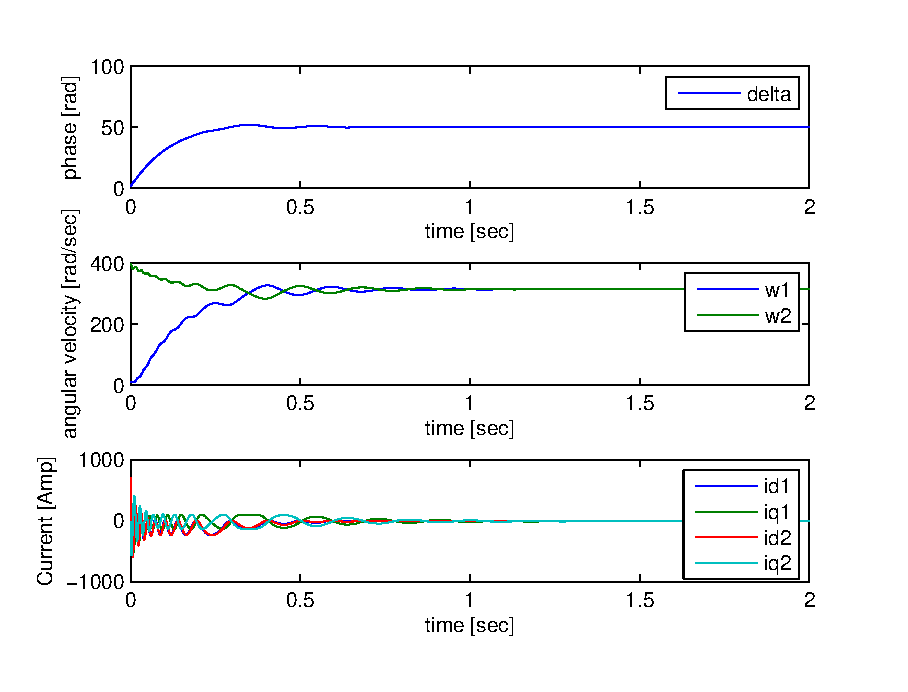
\includegraphics[scale=0.65]{5KWTICSGSimulation} \vspace{-8mm}
\caption{Simulations for TICSG system with 5KW SGs} 
\label{fig:5KWSGTICSGSimulation}
\end{figure}
%%%%%%%%%%**********%%%%%%%%%%**********%%%%%%%%%%**********%%%%%%%%%%

%%%%%%%%%%**********%%%%%%%%%%**********%%%%%%%%%%**********%%%%%%%%%%
\subsection{A stable but non globally stable equilibrium}

Note that Theorem \ref{theorem:TICSGSync} guarantee only local
stability, with $\Emscr$ contained in the region of attraction. 
Figure \ref{fig:InROATICSGSimulation} shows a simulation of a TICSG 
system similar to the previous one, but with smaller $L_s$, for an
initial state which is close enough to $\Emscr$, $\left[z_1(0)\ z_2(0)
\ \delta(0)\right]^\top=\left[40,\ -20,\ 70,\ 400,\ -20,\ 65,\ 0
\right]^\top$, such that the system stabilizes (in particular, the SGs
synchronize). 

Figure \ref{fig:OutROATICSGSimulation} shows another simulation for
the same system, with the initial state $\left[z_1(0)\ z_2(0) \
\delta(0) \right]^\top=\left[-400,\ -200,\ 10,\ 700,\ -20,\ 400,\
1.5708\right]^\top$. \m The simu\-lation indicates that this initial
state is outside the region of attraction, the SGs do not
synchronize. The parameters for the two simulations in this subsection
are (The parameters for the two simulations in this subsection can be found in the appendix,
table \ref{table:TICSGWithLocalE}). 

%\vspace{-4mm}
%%%%%%%%%%**********%%%%%%%%%%**********%%%%%%%%%%**********%%%%%%%%%%
\begin{figure}[ht]
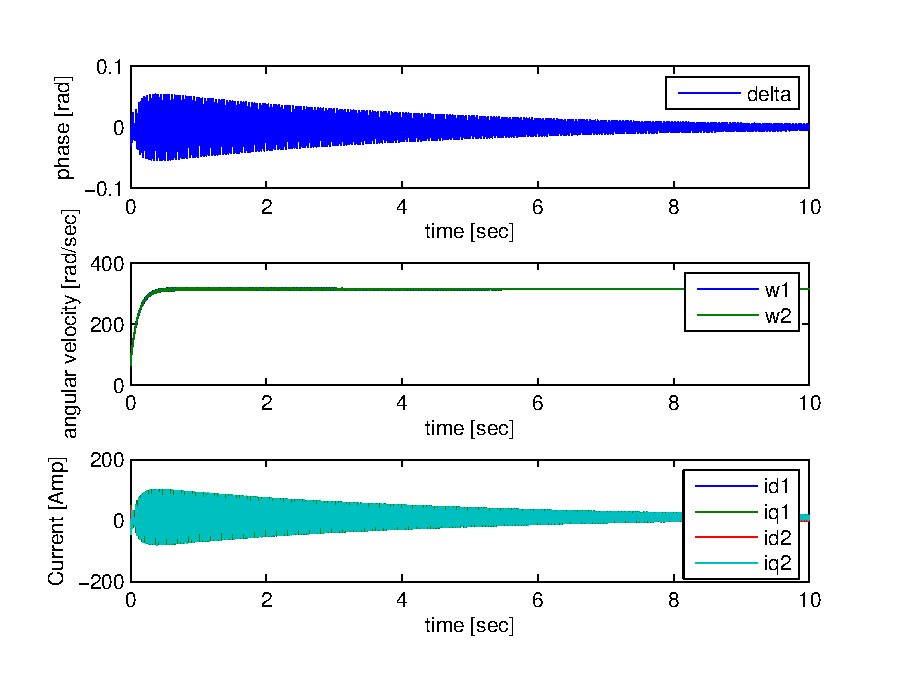
\includegraphics[scale=0.65]{InROATICSGSimulation}
\caption{Simulation for a TICSG system that satisfies the conditions
of Theorem \ref{theorem:TICSGSync}, with initial state inside the 
region of attraction of the stable equilibrium point.}
\label{fig:InROATICSGSimulation}
\end{figure}
%%%%%%%%%%**********%%%%%%%%%%**********%%%%%%%%%%**********%%%%%%%%%%

%\vspace{-4mm}
%%%%%%%%%%**********%%%%%%%%%%**********%%%%%%%%%%**********%%%%%%%%%%
\begin{figure}[ht]
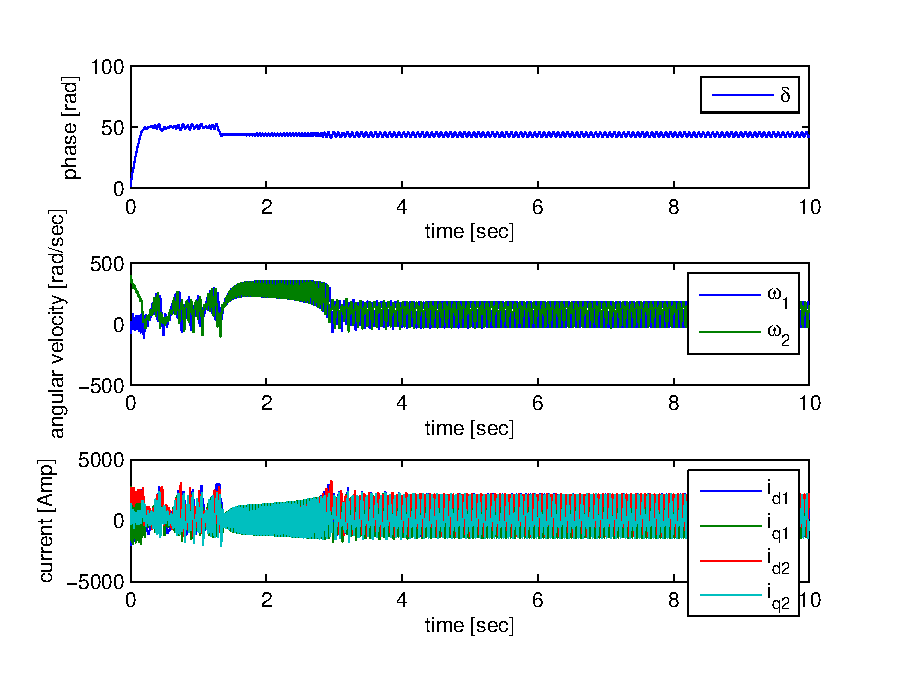
\includegraphics[scale=0.65]{OutROATICSGSimulation}

\caption{Simulation for a TICSG system which satisfy the conditions of
Theorem \ref{theorem:TICSGSync}, with initial state outside the region
of attraction of the stable equilibrium point.}
\label{fig:OutROATICSGSimulation}
\end{figure}
%%%%%%%%%%**********%%%%%%%%%%**********%%%%%%%%%%**********%%%%%%%%%%

%%%%%%%%%%**********%%%%%%%%%%**********%%%%%%%%%%**********%%%%%%%%%%
\subsection{Non stable $\mathscr{E}$ manifold}

%%%%%%%%%%**********%%%%%%%%%%**********%%%%%%%%%%**********%%%%%%%%%%
\begin{figure}[ht]
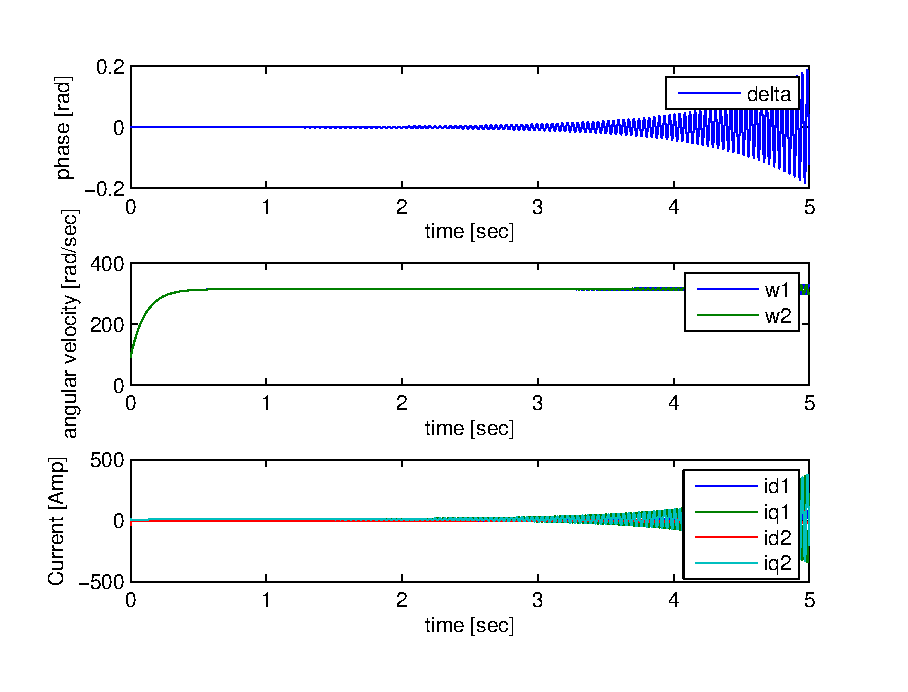
\includegraphics[scale=0.65]{NonStableTICSGSimulation}

\caption{A simulation example with unstable $\Emscr$ manifold}
\label{fig:NonStableTICSGSimulation}
\end{figure}
%%%%%%%%%%**********%%%%%%%%%%**********%%%%%%%%%%**********%%%%%%%%%%

Figure \ref{fig:NonStableTICSGSimulation}, shows an example where the
manifold $\mathscr{E}$ is not locally stable. Simulation of TICSG
system starting form the initial condition $\left[z_1(0)\ z_2(0) \
\delta(0) \right]^\top = \left[ -40, \ 20, \ 90, \ -40, \ 20, \ 90.01,
\ 0 \right]^\top$ do not synchronized. Note that condition
\eqref{eq:eLinearizationLimit} of Theorem \ref{theorem:TICSGSync} does
not hold. (The parameters for these simulations can be found in the appendix,
table \ref{table:TICSGWithNonStableE}).

%%%%%%%%%%++++++++++%%%%%%%%%%++++++++++%%%%%%%%%%++++++++++%%%%%%%%%%
\begin{thebibliography}{99}

\bibitem{AndrieuJayawardhanaPraly} V.~Andrieu, B.~Jayawardhana and L.~Praly, \m On the transverse exponential stability and its use in incremental stability, observer and synchronization. In {\em Proc. of the 52nd IEEE Conference on Decision and Control,
} \m  2013.

\bibitem{AJP_2016} V.~Andrieu, B.~Jayawardhana and L.~Praly, \m 
 Transverse exponential stability and applications, {\em IEEE Trans.
 Automatic Control}, to appear in 2016.

\bibitem{Eitan} E.~Brown, \m {\em A study of the use of synchronverters for grid stabilization using
simulations in SimPower}, MSc thesis, Tel Aviv University, 2015.

\bibitem{CaTa:14} S.Y.~Caliskan and P.~Tabuada, \m
 Compositional transient stability analysis of multimachine 
 power networks, {\em IEEE Trans. Control of Network Systems}, 
 vol.~1, 2014, pp.~4-14.

\bibitem{DoBull:12} F. D{\"o}rfler and F. Bullo, \m 
 \emph{Synchronization and transient stability in power networks and
 nonuniform Kuramoto oscillators}.\hskip 1em plus 0.5em minus 
 0.4em\relax SIAM J. Control and Optim., vol.~50, 2012, 
 pp.~1616-1642.
 
 \bibitem{Fitzgerald:03} A.E.~Fitzgerald, C.~Kingsley and S.D.~Umans,
 \m {\em Electric Machinery}, \m McGraw-Hill, New York, 2003.
 
 \bibitem{GOBS:03}
 M.~Galaz, R.~Ortega, A.S.~Bazanella and A.M.~Stankovic, \m
 An energy-shaping approach to the design of excitation control
 of synchronous generators, {\em Automatica}, vol.~39, 2003,
 pp.~111-119.

\bibitem{GrSt2014} J.J.~Grainger and W.D.~Stevenson,
 {\em Power Systems Analysis}, \m McGraw-Hill, New York, 1994.

\bibitem{GreenProdanovic:07} T.~Green and M.~Prodanovic, \m Control
 of inverter-based micro-grids, {\em Electric Power Systems 
 Research}, vol.~77, 2007, pp.~1204-1213.
 
\bibitem{JayWeissBS:09}
B.~Jayawardhana and G.~Weiss, \m State convergence of passive nonlinear systems with an $L^2$ input,  {\em IEEE Trans. Automatic Control}, 54 (2009), pp.~1723-1727.

\bibitem{Khalil} H.K.~Khalil, \m \emph{Nonlinear Systems} (third 
 edition), Prentice Hall, New Jersey, 2002.
 
\bibitem{Kundur} P.~Kundur, \emph{Power System Stability and Control}.
 \hskip 1em plus 0.5em minus 0.4em\relax McGraw-Hill, New York, 1994.
 
\bibitem{MaWe:15} Y.~Mandel and G.~Weiss, \m Adaptive internal model
 based suppression of torque ripple in brushless DC motor drives,
 {\em Systems Science \& Control Engineering}, vol.~5, 2015, 
 pp.~162-176. 
 
 \bibitem{DePersiSchaft:16} P.~Monshizadeh, C.~De Persis,
 N.~Monshizadeh and A.~van der Schaft, \m Nonlinear Analysis
 of an improved swing equation, \m subm.~2016.
 
\bibitem{NaWe:14} V.~Natarajan and G.~Weiss, \m Almost global 
 asymptotic stability of a constant field current synchronous 
 machine connected to an infinite bus, {\em Proc. of the 53rd 
 IEEE Conf. on Decision and Control}, Los Angeles, CA, Dec. 2014, 
 pp.~3272-3279.

\bibitem{NaWe:15} V.~Natarajan and G.~Weiss, \m Almost global 
 asymptotic stability of a grid-connected synchronous generator,
 submitted in 2015.
 
 %\bibitem{Sastry} S.~Sastry, \emph{Nonlinear Systems}.
 %\hskip 1em plus 0.5em minus 0.4em\relax Springer-Verlag, New York, 1999.

\bibitem{SauerPai1998} P.~W.~Sauer and M.~A.~Pai, \m {\em Power 
 Systems Dynamics and Stability}, Stipes Publishing, Champaign,
 IL, 1997.

\bibitem{SchovanecGilliam1999} L.~Schovanec and D.~Gilliam, \m ODE and PDE lecture notes. {\em The department to Mathematics and Statistics at Texas Tech University. Available at  \url{http://texas.math.ttu.edu/~gilliam/ttu/ode_pde_pdf/Ch4.pdf} 
} \m  1999.

\bibitem{SchovanecGilliam1999} L.~Schovanec and D.~Gilliam, \m ODE
 and PDE lecture notes, {\em The department to Mathematics and 
 Statistics at Texas Tech University.} Available at
 \url{http://texas.math.ttu.edu/~gilliam/ttu/ode_pde_pdf/Ch4.pdf}
 \m 1999.
  
\bibitem{Shafiee_2016} Q.~Shafiee, V.~Nasirian, J.C.~Vasquez, 
 J.M.~Guerrero and A.~Davoudi. \m A multi-functional fully 
 distributed control framework for AC microgrids, {\em 
 IEEE Trans. on Smart Grid}, to appear in 2016.

\bibitem{Schiffer_2016_survey} J.~Schiffer, D.~Zonetti, R.~Ortega,
 A.~Stankovi{\'c}, T.~Sezi  and J.~Raisch, \m A survey on modeling
 of microgrids - from fundamental physics to phasors and voltage 
 sources, {\em Automatica}, vol.~74, 2016, pp.~135-150.

\bibitem{PoDoBu:13} J.W.~Simpson-Porco, F.~D{\"o}rfler
 and F.~Bullo, \m Synchronization and power sharing for
 droop-controlled inverters in islanded microgrids, {\em 
 Automatica}, vol.~49, 2013, pp.~2603-2611.

\bibitem{Walker:94} J.H.~Walker, \m {\em Large Synchronous Machines: 
 Design, Manufacture and Operation}, \m Oxford University Press, 
 Oxford, 1981.

 \bibitem{Zhong:13} Q.-C.~Zhong, \m Robust droop controller for 
 accurate proportional load sharing among inverters operated in 
 parallel, {\em IEEE Trans. on Industrial Electronics}, vol.~60,
 2013, pp.~1281-1290.


\bibitem{ZhWe:11} Q.-C.~Zhong and G.~Weiss, \m Synchronverters: 
 Inverters that mimic synchronous generators, {\em IEEE Trans. 
 Industr. Electronics}, vol.~58, 2011, pp.~1259-1267.

\bibitem{ZhouOhsawa2009} J.~Zhou and Y.~Ohsawa, \m Improved swing
 equation and its properties in synchronous generators, {\em
 IEEE Trans. Circuits and Systems I}, vol.~56, 2009, pp.~200-209.

\end{thebibliography}

\appendix
\chapter{appendix \label{chap:Appendix}}
\section{Synchronous generator parameters\label{chap:Appendix}}

\subsection*{5 KW SG}

The parameters of 5KW SG are taken from \cite{Eitan}

\begin{table}[H]
\begin{tabular}{|c|c|}
\hline 
Variable & Value\tabularnewline
\hline 
\hline 
$J$ & $0.2\qquad[kg\cdot m^{2}]$\tabularnewline
\hline 
$D_{p}$ & $1.7\qquad\left[J\cdot sec\right]$\tabularnewline
\hline 
$R_{s}$ & $0.152\qquad\left[\Omega\right]$\tabularnewline
\hline 
$L_{s}$ & $4.4\qquad\left[mH\right]$\tabularnewline
\hline 
$mi_{f}$ & $1.05\qquad\left[V\cdot sec\right]$\tabularnewline
\hline 
$\omega_{g}$ & $60\cdotp2\cdotp\pi\qquad\left[\frac{rad}{sec}\right]$\tabularnewline
\hline 
$V$ & $330\qquad\left[V\right]$\tabularnewline
\hline 
$P_{m}$ & $5\qquad\left[kW\right]$\tabularnewline
\hline 
\end{tabular}\caption{Parameters for 5KW SG}
\label{table:5KWSG}
\end{table}


\subsection*{1 MW SG}

The parameters of 1MW SG are taken from \cite{Eitan}

\begin{table}[H]
\begin{tabular}{|c|c|}
\hline 
Variable & Value\tabularnewline
\hline 
\hline 
$J$ & $40.05\qquad[kg\cdot m^{2}]$\tabularnewline
\hline 
$D_{p}$ & $337\qquad\left[J\cdot sec\right]$\tabularnewline
\hline 
$R_{s}$ & $0.4\qquad\left[m\Omega\right]$\tabularnewline
\hline 
$L_{s}$ & $18\qquad\left[mH\right]$\tabularnewline
\hline 
$mi_{f}$ & $1.79\qquad\left[V\cdot sec\right]$\tabularnewline
\hline 
$\omega_{g}$ & $60\cdotp2\cdotp\pi\qquad\left[\frac{rad}{sec}\right]$\tabularnewline
\hline 
$V$ & $563\qquad\left[V\right]$\tabularnewline
\hline 
$P_{m}$ & $1\qquad\left[MW\right]$\tabularnewline
\hline 
\end{tabular}\caption{Parameters for 1MW SG}
\label{table:1MWSG}
\end{table}


\subsection*{Example for SG parameters which leads to different behavior for the
reduced model}

This set of parameters shows different behavior of the FOM model
and for the improved swing equation model. This set of parameters
is basically the 5KW SG parameters set which connected to grid with
lower voltage and fed by $50$ {[}KW{]} prime mover. 

\begin{table}[H]
\begin{tabular}{|c|c|}
\hline 
Variable & Value\tabularnewline
\hline 
\hline 
$J$ & $0.2\qquad[kg\cdot m^{2}]$\tabularnewline
\hline 
$D_{p}$ & $1.7\qquad\left[J\cdot sec\right]$\tabularnewline
\hline 
$R_{s}$ & $0.152\qquad\left[\Omega\right]$\tabularnewline
\hline 
$L_{s}$ & $4.4\qquad\left[mH\right]$\tabularnewline
\hline 
$mi_{f}$ & $1.05\qquad\left[V\cdot sec\right]$\tabularnewline
\hline 
$\omega_{g}$ & $60\cdotp2\cdotp\pi\qquad\left[\frac{rad}{sec}\right]$\tabularnewline
\hline 
$V$ & $200\qquad\left[V\right]$\tabularnewline
\hline 
$P_{m}$ & $50\qquad\left[kW\right]$\tabularnewline
\hline 
\end{tabular}\caption{Parameters for SG which leads to different behavior for the reduced
model}
\label{table:DifferentBehaviorParamsSetSG}
\end{table}


\subsection*{Example for SG parameters which leads to different behavior for the
reduced model}

This set of parameters shows different region of attraction of the
FOM model and for the improved swing equation model. This set of
parameters is basically the 5KW SG parameters set with stronger $i_{f}$
(or stronger permanent magnet).

\begin{table}[H]
\begin{tabular}{|c|c|}
\hline 
Variable & Value\tabularnewline
\hline 
\hline 
$J$ & $0.2\qquad[kg\cdot m^{2}]$\tabularnewline
\hline 
$D_{p}$ & $1.7\qquad\left[J\cdot sec\right]$\tabularnewline
\hline 
$R_{s}$ & $0.152\qquad\left[\Omega\right]$\tabularnewline
\hline 
$L_{s}$ & $1.05\qquad\left[mH\right]$\tabularnewline
\hline 
$mi_{f}$ & $3.5\qquad\left[V\cdot sec\right]$\tabularnewline
\hline 
$\omega_{g}$ & $60\cdotp2\cdotp\pi\qquad\left[\frac{rad}{sec}\right]$\tabularnewline
\hline 
$V$ & $330\qquad\left[V\right]$\tabularnewline
\hline 
$P_{m}$ & $5\qquad\left[kW\right]$\tabularnewline
\hline 
\end{tabular}\caption{Parameters for SG which leads to different region of attraction}
\label{table:DifferentRegionOfAttraction}
\end{table}

\subsection*{Parameters for TICSG system with local  $\mathcal{E}$ manifold}

\begin{table}[H]
\begin{tabular}{|c|c|}
\hline 
Variable & Value\tabularnewline
\hline 
\hline 
$J$ & $0.2\qquad[kg\cdot m^{2}]$\tabularnewline
\hline 
$D_{p}$ & $1.7\qquad\left[J\cdot sec\right]$\tabularnewline
\hline 
$R_{s}$ & $11\qquad\left[m\Omega\right]$\tabularnewline
\hline 
$L_{s}$ & $0.4\qquad\left[mH\right]$\tabularnewline
\hline 
$mi_{f}$ & $-1.38\qquad\left[V\cdot sec\right]$\tabularnewline
\hline 
$R_L$ & $18.86\qquad\left[\Omega\right]$\tabularnewline
\hline 
$T_m$ & $549.9254\qquad\left[N\cdot m\right]$\tabularnewline
\hline 

\end{tabular}\caption{Parameters TICSG system with local  $\mathcal{E}$}
\label{table:TICSGWithLocalE}
\end{table}

\subsection*{Parameters for TICSG system with non stable  $\mathcal{E}$ manifold}

\begin{table}[H]
\begin{tabular}{|c|c|}
\hline 
Variable & Value\tabularnewline
\hline 
\hline 
$J$ & $0.2\qquad[kg\cdot m^{2}]$\tabularnewline
\hline 
$D_{p}$ & $1.7\qquad\left[J\cdot sec\right]$\tabularnewline
\hline 
$R_{s}$ & $11\qquad\left[m\Omega\right]$\tabularnewline
\hline 
$L_{s}$ & $0.35\qquad\left[mH\right]$\tabularnewline
\hline 
$mi_{f}$ & $-1.38\qquad\left[V\cdot sec\right]$\tabularnewline
\hline 
$R_L$ & $18.86\qquad\left[\Omega\right]$\tabularnewline
\hline 
$T_m$ & $549.9254\qquad\left[N\cdot m\right]$\tabularnewline
\hline 

\end{tabular}\caption{Parameters for TICSG system with non stable  $\mathcal{E}$ manifold}
\label{table:TICSGWithNonStableE}
\end{table}

\section{Proof that for the TICSG, rank$\left[M|n\right]=3$, assuming that  $\sin\delta_{0}=0$ \label{chap:AppendixProof}}

\[
M=\left[\begin{array}{cc}
-R_{tot} & -R_{L}\cos\delta^{e}\\
-\omega^{e}L_{s} & -R_{L}\sin\delta^{e}\\
-R_{L}\cos\delta^{e} & -R_{tot}\\
R_{L}\sin\delta^{e} & -\omega^{e}L_{s}
\end{array}\right]
\]

and 

\[
n=\left[\begin{array}{c}
i_{q}^{e}\left(\omega^{e}L_{s}+R_{L}\sin\delta^{e}\right)\\
-mi_{f}\omega^{e}-i_{q}^{e}\left(R_{tot}+R_{L}\cos\delta^{e}\right)\\
i_{q}^{e}\left(\omega^{e}L_{s}-R_{L}\sin\delta^{e}\right)\\
-mi_{f}\omega^{e}-i_{q}^{e}\left(R_{tot}+R_{L}\cos\delta^{e}\right)
\end{array}\right]
\]

Denote $\alpha=\omega_{0}L_{s}+R_{L}\sin\delta_{0}$ and $\beta=\omega_{0}L_{s}-R_{L}\sin\delta_{0}$,
then:

\begin{equation}
\left[M|n\right]=\left[\begin{array}{ccc}
-R_{tot} & \quad-R_{L}\cos\delta^{e}\quad & i_{q}^{e}\alpha\\
-\omega^{e}L_{s} & \quad-R_{L}\sin\delta^{e}\quad & -mi_{f}\omega^{e}-i_{q}^{0}\left(R_{tot}+R_{L}\cos\delta^{e}\right)\\
-R_{L}\cos\delta^{e} & \quad-R_{tot}\quad & i_{q}^{e}\beta\\
R_{L}\sin\delta^{e} & \quad-\omega^{e}L_{s}\quad & -mi_{f}\omega^{e}-i_{q}^{0}\left(R_{tot}+R_{L}\cos\delta^{e}\right)
\end{array}\right]\label{eq:M_n}
\end{equation}


\subsubsection*{Case A: $\alpha=0$ and $\beta=0$}

Because $\alpha=0$ and $\beta=0$ it means that $\omega^{e}L_{s}+R_{L}\sin\delta^{e}=\omega^{e}L_{s}-R_{L}\sin\delta^{e}$ 
and hence $R_{L}\sin\delta^{e}=0$ which contradicts our assumption.

\subsubsection*{Case B: $\alpha=0$ and $\beta\protect\ne0$}

Lets define 

\begin{equation}
T=\left[\begin{array}{cccc}
0 & 0 & 1 & 0\\
1 & 0 & 0 & 0\\
0 & 1 & 0 & -1
\end{array}\right]\left[M|n\right]=\left[\begin{array}{ccc}
-R_{L}\cos\delta^{e} & -R_{tot} & i_{q}^{e}\beta\\
-R_{tot} & -R_{L}\cos\delta^{e} & 0\\
0 & \beta & 0
\end{array}\right].\label{eq:MATRIX_1}
\end{equation}

Now, if $\cos\delta^{e}=0$ then rank$(T)=3$. If $\cos\delta^{e}\ne0$
we define 

\[
T_{2}=\left[\begin{array}{ccc}
1 & 0 & 0\\
0 & \beta & -R_{L}\cos\delta^{e}\\
0 & 0 & 1
\end{array}\right]T=\left[\begin{array}{ccc}
-R_{L}\cos\delta_{0} & -R_{tot} & i_{q}^{e}\beta\\
-R_{tot}\beta & 0 & 0\\
0 & \beta & 0
\end{array}\right]
\]

it is easy to see that rank$(T_{2})=3$.

\subsubsection*{Case C: $\alpha\protect\ne0$ and $\beta=0$}

Lets define

\begin{equation}
T_{3}=\left[\begin{array}{cccc}
1 & 0 & 0 & 0\\
0 & 0 & 1 & 0\\
0 & 1 & 0 & -1
\end{array}\right]\left[M|n\right]=\left[\begin{array}{ccc}
-R_{tot} & -R_{L}\cos\delta^{e} & i_{q}^{e}\alpha\\
-R_{L}\cos\delta^{e} & -R_{tot} & 0\\
-\alpha & 0 & 0
\end{array}\right]\label{eq:MATRIX_2}
\end{equation}

it is easy to see that rank$(T_{3})=3$.

\subsubsection*{Case D: $\alpha\protect\ne0$ and $\beta\protect\ne0$}

Lets define

\begin{equation}
T_{4}=\left[\begin{array}{cccc}
1 & 0 & 0 & 0\\
\alpha & 0 & \beta & 0\\
0 & 1 & 0 & -1
\end{array}\right]\left[M|n\right]=\left[\begin{array}{ccc}
-R_{tot} & -R_{L}\cos\delta^{e} & i_{q}^{e}\alpha\\
\frac{R_{L}\cos\delta^{e}}{\beta}-\frac{R_{tot}}{\alpha} & -\frac{R_{L}\cos\delta^{e}}{\alpha}+\frac{R_{tot}}{\beta} & 0\\
-\alpha & \beta & 0
\end{array}\right].\label{eq:MATRIX_4}
\end{equation}

It is impossible that both $-\frac{R_{L}\cos\delta^{e}}{\alpha}+\frac{R_{tot}}{\beta}=0$
and $\frac{R_{L}\cos\delta^{e}}{\beta}-\frac{R_{tot}}{\alpha}=0$
because it implies that 
$$\left\{ \begin{array}{c}
-\beta R_{L}\cos\delta^{e}+\alpha R_{tot}=0\\
\alpha R_{L}\cos\delta^{e}-\beta R_{tot}=0
\end{array}\right..$$ 

By subtract the first equation from the second we get 

$(\alpha+\beta)R_{L}\cos\delta^{e}=(\alpha+\beta)R_{tot}$, which is impossible because  $\alpha+\beta=2\omega^{e}L_{s}>0$ and $R_{tot}=R_L+R_s>R_{L}\cos\delta^{e}$.



If $-\frac{R_{L}\cos\delta_{0}}{\alpha}+\frac{R_{tot}}{\beta}=0$ and $\frac{R_{L}\cos\delta^{e}}{\beta}-\frac{R_{tot}}{\alpha} \neq 0$,
then it is easy to see that rank$(T_{4})=3$.

If $-\frac{R_{L}\cos\delta_{0}}{\alpha}+\frac{R_{tot}}{\beta}\ne0$
we define

\[
\begin{array}{c}
T_{5}=\left[\begin{array}{ccc}
1 & 0\quad & 0\\
0 & 0\quad & 1\\
0 & -\beta \quad & -\frac{R_{L}\cos\delta_{0}}{\alpha}+\frac{R_{tot}}{\beta}
\end{array}\right]T_{4}=\\
\left[\begin{array}{ccc}
-R_{tot} & -R_{L}\cos\delta^{e} & i_{q}^{e}\alpha\\
-\alpha & \beta & 0\\
R_{tot} \left( \frac{\beta}{\alpha}- \frac{\alpha}{\beta}\right) & 0 & 0
\end{array}\right]
\end{array}
\]

because $ \alpha \neq \beta$, rank$(T_{5})=3$. 

We show that for any possible case, after applying linear
transformation on $\left[M|n\right]$ the resulting rank is 3. 

\newpage{}

\end{document}
